\documentclass[conference]{IEEEtran}
\usepackage[utf8]{inputenc}
\usepackage[T1]{fontenc}
\usepackage[spanish,es-nodecimaldot]{babel}
\usepackage{textcomp,graphicx,booktabs,amsmath,float,url,cite}
\graphicspath{{../}{./}} % figuras en ../figures (repositorio) o ./figures (Overleaf)
\def\UrlBreaks{\do\/\do\-\do\.\do\_}
\Urlmuskip=0mu plus 1mu

\begin{document}

\title{Predicción horaria de PM$_{2{,}5}$ en Santa Anita:\\ aporte de las variables de calendario}

\author{
\IEEEauthorblockN{Jobeth Alexander León Pantaleón}
\IEEEauthorblockA{Sistemas de Información\\UTEC, Lima, Perú\\Jobeth.leon@utec.pe}
\and
\IEEEauthorblockN{Josué Yeremi Huamán Huamaní}
\IEEEauthorblockA{Ciencias de la Computación\\UTEC, Lima, Perú\\josue.huaman.h@utec.edu.pe}
\and
\IEEEauthorblockN{Enrique Zheng Chan}
\IEEEauthorblockA{Ciencias de la Computación\\UTEC, Lima, Perú\\enrique.zheng@utec.edu.pe}
\and
\IEEEauthorblockN{Requelmy Limaco Porras}
\IEEEauthorblockA{Departamento de Ingeniería\\UTEC, Lima, Perú\\requelmy.limaco@utec.edu.pe}
}

\maketitle

\begin{abstract}
Este trabajo predice la concentración de PM$_{2{,}5}$ de la siguiente hora en la estación Santa Anita de SENAMHI (Lima Metropolitana) a partir de su historial reciente, y evalúa si las variables de calendario aportan por encima de ese historial. Se usan 19.391 mediciones horarias disponibles entre enero de 2022 y abril de 2024, una partición cronológica en entrenamiento, validación y prueba, ajuste de hiperparámetros por validación temporal y comprobaciones explícitas de fuga de información. Se comparan una línea base de persistencia, Ridge y Lasso, Random Forest y HistGradientBoosting. En prueba (enero--abril de 2024), los modelos de árboles reducen el MAE de la persistencia en 14--15~\% (2,41 y 2,43 frente a 2,83~\textmu g/m\textsuperscript{3}) y Ridge en 7~\%. El calendario mejora a los árboles entre 2 y 3~\% en validación, gracias a la hora del día, pero no a los modelos lineales, y el día de la semana no aporta. En el decil superior de concentraciones el error es de dos a cuatro veces el del resto y todos los modelos subestiman los valores sobre 50~\textmu g/m\textsuperscript{3}. El historial propio de la serie permite mejoras consistentes pero modestas a una hora, y sin variables meteorológicas no basta para anticipar los episodios altos. Código: \url{https://github.com/AIexander-lx/prediccion-pm25-santa-anita-}.
\end{abstract}

\begin{IEEEkeywords}
PM2.5, calidad del aire, predicción horaria, Machine Learning, series temporales, Lima.
\end{IEEEkeywords}

% Sección 2 de la guía (Introducción y formulación del problema). Rol 4.
\section{Introducción y formulación del problema}
\label{sec:intro}

\subsection{Motivación}
El material particulado fino PM$_{2{,}5}$, formado por partículas de diámetro aerodinámico menor o igual a 2,5~\textmu m, es uno de los indicadores más usados para estudiar la calidad del aire. Su exposición se asocia con efectos adversos sobre la salud, por lo que existen valores de referencia para el promedio de 24 horas: 50~\textmu g/m\textsuperscript{3} en el Estándar de Calidad Ambiental (ECA) peruano~\cite{minam_eca_2017} y 15~\textmu g/m\textsuperscript{3} en la guía de la OMS de 2021~\cite{who_aqg_2021}. En la estación Santa Anita, de la zona este de la red de SENAMHI en Lima Metropolitana~\cite{senamhi_vigilancia_2021}, el 93~\% de los días con cobertura suficiente entre 2022 y 2024 supera la guía de la OMS y el 10,3~\% el ECA, lo que da sentido a disponer de un pronóstico a corto plazo.

Este trabajo predice la concentración de PM$_{2{,}5}$ de la \emph{siguiente hora} en esa estación a partir de su historial reciente. El pronóstico se compara con la persistencia, que supone que la siguiente hora será igual a la actual y es la referencia habitual en pronóstico~\cite{hyndman2021fpp3}. Además se estudia si la hora del día y el día de la semana aportan información por encima del historial, y qué ocurre con los errores cuando la concentración es alta.

\subsection{Trabajos previos}
La predicción de PM$_{2{,}5}$ en Lima ya se ha abordado con aprendizaje automático. Hoyos Cordova et al.~\cite{hoyos2021} predijeron la hora siguiente en cinco estaciones de SENAMHI con redes MLP y LSTM, y observaron que el desempeño empeora en los episodios críticos. Oblitas y Escobedo~\cite{oblitas2024xgboost} usaron XGBoost y LightGBM en San Borja y vieron que excluir variables relevantes reduce la precisión. Solis Teran et al.~\cite{solis2025} compararon nueve enfoques estadísticos y neuronales, y encontraron que modelos como ARIMA pueden superar a una LSTM cuando la serie tiene estacionalidad y pocas observaciones, de modo que no conviene suponer que el modelo más complejo será el mejor. No encontramos un estudio horario centrado en Santa Anita, por lo que este trabajo aporta evidencia sobre una estación de la zona este, con una persistencia como referencia, una evaluación que respeta el orden temporal~\cite{bergmeir2012} y un análisis de errores en los episodios altos.

\subsection{Objetivo, tarea y preguntas de investigación}
El objetivo es desarrollar y evaluar modelos que predigan la concentración de PM$_{2{,}5}$ una hora adelante en Santa Anita. Es una tarea de \emph{regresión supervisada}: la salida es un valor numérico y los registros históricos relacionan la información disponible en la hora $t$ con la concentración observada en $t+1$. Las preguntas de investigación son:
\begin{itemize}
\item \textbf{PI1.} ¿Cuánto mejora un modelo de aprendizaje automático sobre la persistencia como pronóstico a una hora?
\item \textbf{PI2.} ¿Aportan la hora del día y el día de la semana por encima de lo que ya contiene el historial reciente de la serie?
\item \textbf{PI3.} ¿Se degrada el desempeño en el régimen de concentraciones altas, el de mayor relevancia sanitaria?
\end{itemize}
La hipótesis de partida para PI2 es que el calendario puede representar patrones que el historial no captura por completo; el EDA solo muestra diferencias descriptivas, por lo que su utilidad debe comprobarse con la reducción del error en datos posteriores a los de entrenamiento. PI3 se apoya en lo observado por Hoyos Cordova et al.~\cite{hoyos2021}. Las conclusiones se limitan a esta estación y a este periodo.

\subsection{Contribuciones y organización}
El trabajo aporta (i)~un conjunto supervisado sin fuga de información, con comprobaciones explícitas, (ii)~una comparación de persistencia, Ridge, Lasso, Random Forest y HistGradientBoosting con ajuste por validación temporal, (iii)~una respuesta con intervalos de confianza a las tres preguntas y (iv)~un análisis de errores por hora, mes y nivel de concentración. El código, los datos procesados y las figuras están en el repositorio público\footnote{\url{https://github.com/AIexander-lx/prediccion-pm25-santa-anita-}}. La sección~\ref{sec:eda} describe los datos y el EDA; las secciones~\ref{sec:preproc} a~\ref{sec:diseno}, el preprocesamiento, los modelos y el diseño experimental; la sección~\ref{sec:resultados}, los resultados; y las secciones~\ref{sec:discusion} y~\ref{sec:conclusiones}, la discusión y las conclusiones.


\section{Datos y análisis exploratorio}
\label{sec:eda}
% Subsecciones iniciales de la sección 3 (de la entrega P1, condensadas). Rol 4.
\subsection{Fuente y descripción del dataset}
\label{sec:fuente}
Los datos provienen de SENAMHI y están publicados en la Plataforma Nacional de Datos Abiertos como ``Monitoreo de los contaminantes del aire en Lima Metropolitana''~\cite{senamhi_datos_2025}, con licencia Open Data Commons Attribution. Se usa el archivo filtrado a la estación Santa Anita, con 82.542 registros y 15 columnas entre enero de 2015 y mayo de 2024; se verificó que coincide con los registros de esa estación en el archivo completo de la red. Cada fila contiene identificador, estación, fecha y hora, ubicación, concentraciones de PM$_{10}$, PM$_{2{,}5}$ y NO$_2$ (columna \texttt{PM2\_5} para la variable de interés) y datos administrativos. Por tipo, la fecha y hora es temporal, las tres concentraciones son numéricas continuas, y el identificador, la estación y los datos administrativos son categóricos o de texto; la variable objetivo es PM$_{2{,}5}$ en la hora siguiente (regresión, por lo que no hay clases que balancear). El diccionario no indica la unidad; el informe de vigilancia de SENAMHI~\cite{senamhi_vigilancia_2021} reporta estos contaminantes en \textmu g/m\textsuperscript{3}, unidad que se adopta. Los identificadores, la ubicación y la fecha de corte no se usan como predictores, porque no describen el comportamiento del contaminante en una única estación.

\subsection{Selección de la estación y del periodo}
\label{sec:periodo}
Se trabaja con una sola estación para mantener una referencia geográfica constante; los resultados no representan a toda Lima. La disponibilidad de PM$_{2{,}5}$ varía mucho entre años: entre 84,6~\% y 94,3~\% en 2015--2017, y luego 50,2~\% en 2018, 20,9~\% en 2019, 0~\% en 2020 y 3,5~\% en 2021, hasta volver a 94,0~\%, 95,0~\% y 97,7~\% en 2022, 2023 y enero--mayo de 2024. Por ello se eligió el tramo continuo más reciente con alta disponibilidad, del 1 de enero de 2022 al 30 de abril de 2024, sin registros duplicados por fecha y hora. Comprende 20.424 horas, de las cuales 19.391 (94,94~\%) tienen medición de PM$_{2{,}5}$. Esta elección introduce un sesgo: el conjunto corresponde a los años en que la estación funcionó con normalidad y excluye el periodo de 2020, y dos años completos más cuatro meses caracterizan limitadamente la variación entre años.

% Sección 3 (EDA), continuación de las subsecciones de P1 (fuente, selección de
% estación y periodo). Se inserta con % Sección 3 (EDA), continuación de las subsecciones de P1 (fuente, selección de
% estación y periodo). Se inserta con % Sección 3 (EDA), continuación de las subsecciones de P1 (fuente, selección de
% estación y periodo). Se inserta con \input{seccion_3_eda} después de ellas.
% Figuras esperadas en figures/ (las mismas de la notebook 01_eda).

\subsection{Calidad de los datos y valores faltantes}
\label{sec:faltantes}

De las 20.424 horas del periodo, 1.033 (5,06~\%) no tienen medición de PM2.5. Esa cifra agregada describe mal el problema: las ausencias se agrupan en 47 interrupciones con una mediana de 11 horas, y las 12 que duran 24 horas o más concentran 700 horas, el 68~\% de todos los faltantes (la mayor dura 126 horas). El archivo no documenta la causa, por lo que no puede asumirse que los faltantes sean aleatorios. Si coincidieran con episodios de alta concentración, los estadísticos descriptivos subestimarían los valores extremos. Por eso no se imputa ni se interpola ningún valor: las horas sin medición se conservan explícitamente en la serie.

Se aplicaron tres controles de coherencia. Ninguna de las 18.671 horas con PM2.5 y PM10 simultáneos presenta PM2.5 por encima de PM10, la racha máxima de valores idénticos consecutivos es de 2 (descarta un sensor bloqueado) y se observaron 49 variaciones horarias superiores a 50~\textmu g/m\textsuperscript{3}, con un máximo de 121,0. Estas últimas se señalan para revisión, pero no se descartan.

\subsection{Distribución y valores extremos}
\label{sec:distribucion}

La serie disponible (19.391 mediciones) tiene media de 29,29 y mediana de 24,50~\textmu g/m\textsuperscript{3}, desviación estándar de 18,17, percentil 95 de 65,31 y máximo de 191,5. La asimetría es de 2,11: una minoría de horas con concentraciones altas arrastra el promedio. Al ser la variable objetivo continua, no existe un desbalance de clases en sentido estricto, pero la distribución produce un efecto equivalente, porque las concentraciones altas están poco representadas.

La regla de 1,5 veces el rango intercuartílico señala 1.126 mediciones (5,81~\%). No se eliminan: el 95~\% corresponde a 2022, se concentran entre mayo y octubre y entre las 12:00 y las 16:00, que es la franja de mayor mediana horaria. Un error instrumental no reproduciría esa estructura estacional y horaria, de modo que la evidencia favorece interpretarlas como episodios reales de contaminación, que además son las horas de mayor relevancia sanitaria. Como contexto, de los 795 días con al menos 18 horas medidas, el 93~\% supera la guía diaria de la OMS (15~\textmu g/m\textsuperscript{3}) y el 10,3~\% el estándar peruano (50~\textmu g/m\textsuperscript{3}).

\subsection{Patrón diario y cambio de régimen}
\label{sec:regimen}

La mediana horaria alcanza su máximo a las 14:00 (34,4~\textmu g/m\textsuperscript{3}) y su mínimo a las 22:00 (17,0), por lo que la hora del día está asociada al nivel de PM2.5. Esta es una diferencia descriptiva; que mejore la predicción debe comprobarse con modelos.

El nivel medio desciende a lo largo del periodo: 38,8~\textmu g/m\textsuperscript{3} en 2022, 23,8 en 2023 y 17,7 en enero–abril de 2024. Parte de la caída de 2024 es estacional, pero 2022 supera a 2023 en 11 de los 12 meses, con una diferencia concentrada entre mayo y octubre, de modo que el calendario no la explica por completo (Fig.~\ref{fig:regimen}). Una partición cronológica entrena entonces en un régimen de concentraciones más altas que el de evaluación, y el error absoluto no es comparable entre tramos; las métricas deberán reportarse por separado para cada bloque.

\begin{figure}[t]
\centering
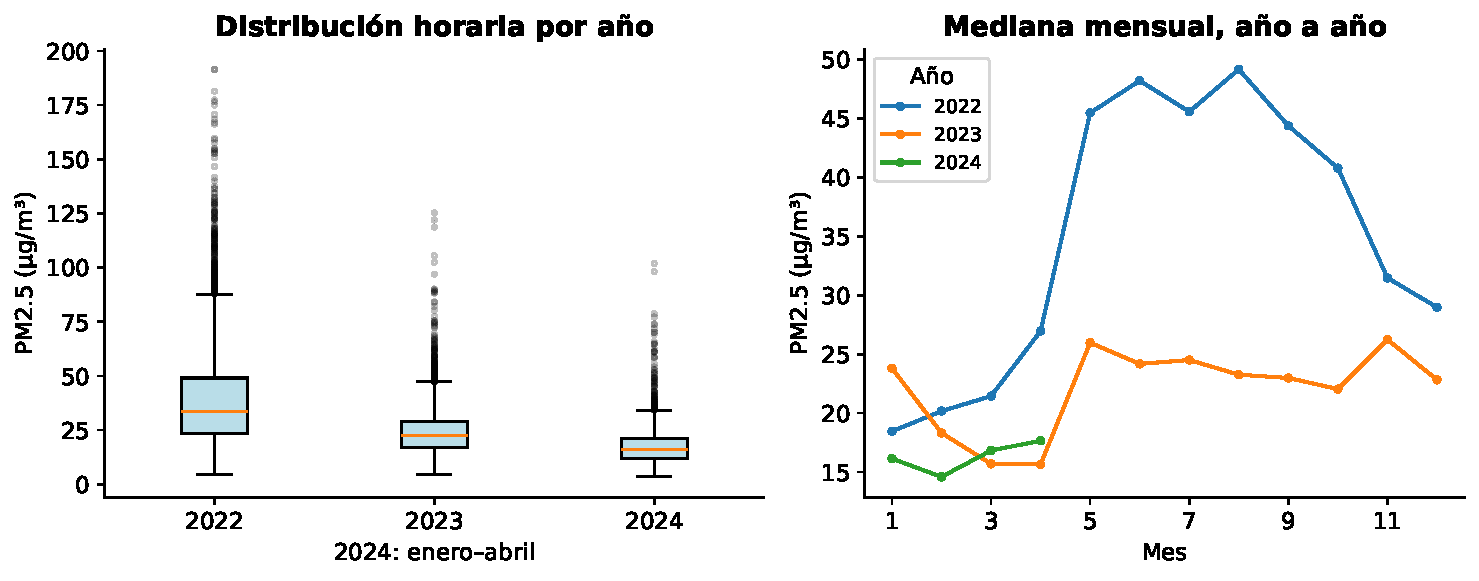
\includegraphics[width=\columnwidth]{figures/12_distribucion_anual.pdf}
\caption{Cambio de nivel entre años y comparación de medianas mensuales.}
\label{fig:regimen}
\end{figure}

\subsection{Dependencia temporal}
\label{sec:autocorrelacion}

Entre horas consecutivas la correlación de Pearson es de 0,912 (19.343 pares completos). La autocorrelación cae a 0,464 en el rezago 12 y vuelve a subir a 0,651 en el rezago 24, lo que muestra el ciclo diario. La autocorrelación parcial se concentra en el primer rezago (0,912), es negativa en el segundo ($-0{,}184$) y no supera 0,12 en valor absoluto entre los rezagos 3 y 24 (Fig.~\ref{fig:acf}). Los rezagos inmediatos aportan la información propia de corto plazo, mientras que el repunte a 24 horas corresponde al ciclo diario y puede representarse con variables de calendario en lugar de decenas de rezagos. Cuál de las dos opciones rinde más se responde comparando modelos con y sin calendario (PI2).

\begin{figure}[t]
\centering
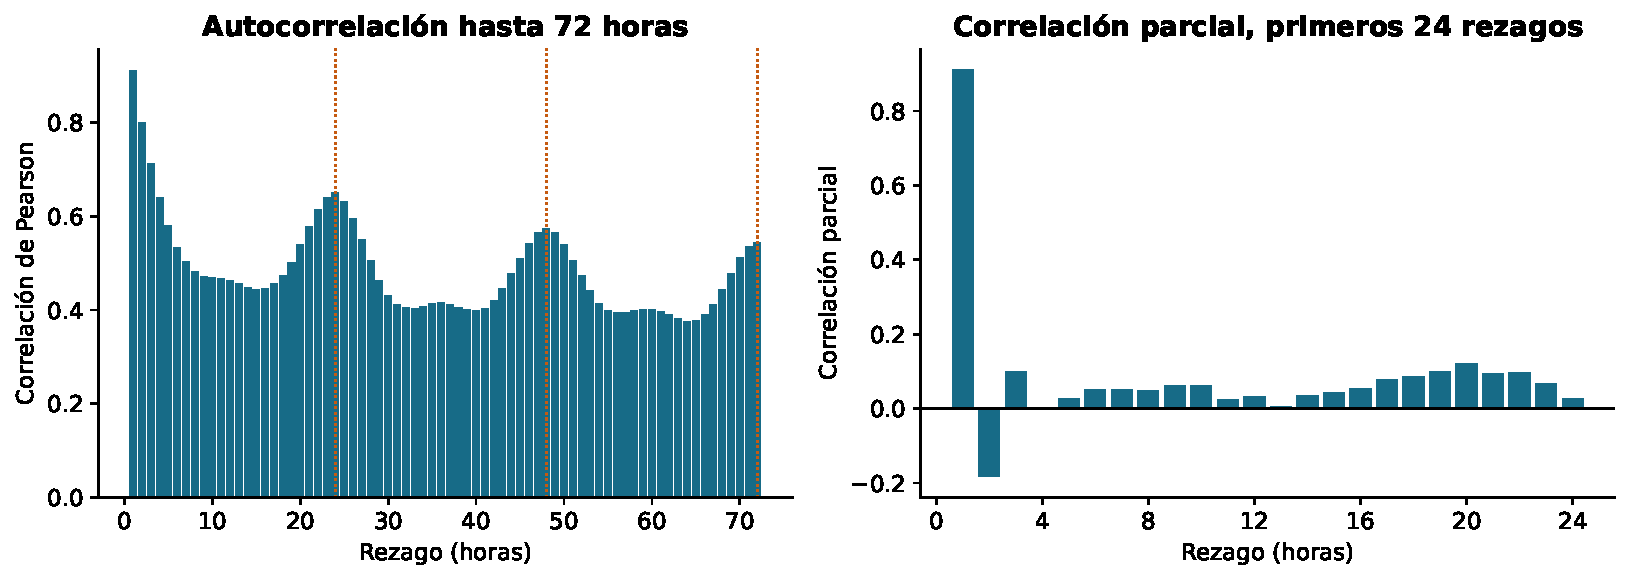
\includegraphics[width=\columnwidth]{figures/13_autocorrelacion.pdf}
\caption{Autocorrelación y autocorrelación parcial de PM2.5 hasta 48 horas, calculadas con las horas en que ambos valores están disponibles.}
\label{fig:acf}
\end{figure}

\subsection{Implicaciones para el modelado}
\label{sec:implicaciones}

El análisis exploratorio condiciona el diseño de la segunda etapa en cuatro puntos: los faltantes se agrupan en tramos y no se imputan, por lo que cada hora utilizable exige respuesta e historial completos; los valores extremos se conservan; la partición debe ser cronológica y sus métricas desagregadas por bloque, por el cambio de régimen; y el baseline natural es la persistencia, dada la correlación de 0,912 a una hora. Estas decisiones se concretan en la sección~\ref{sec:preproc}.
 después de ellas.
% Figuras esperadas en figures/ (las mismas de la notebook 01_eda).

\subsection{Calidad de los datos y valores faltantes}
\label{sec:faltantes}

De las 20.424 horas del periodo, 1.033 (5,06~\%) no tienen medición de PM2.5. Esa cifra agregada describe mal el problema: las ausencias se agrupan en 47 interrupciones con una mediana de 11 horas, y las 12 que duran 24 horas o más concentran 700 horas, el 68~\% de todos los faltantes (la mayor dura 126 horas). El archivo no documenta la causa, por lo que no puede asumirse que los faltantes sean aleatorios. Si coincidieran con episodios de alta concentración, los estadísticos descriptivos subestimarían los valores extremos. Por eso no se imputa ni se interpola ningún valor: las horas sin medición se conservan explícitamente en la serie.

Se aplicaron tres controles de coherencia. Ninguna de las 18.671 horas con PM2.5 y PM10 simultáneos presenta PM2.5 por encima de PM10, la racha máxima de valores idénticos consecutivos es de 2 (descarta un sensor bloqueado) y se observaron 49 variaciones horarias superiores a 50~\textmu g/m\textsuperscript{3}, con un máximo de 121,0. Estas últimas se señalan para revisión, pero no se descartan.

\subsection{Distribución y valores extremos}
\label{sec:distribucion}

La serie disponible (19.391 mediciones) tiene media de 29,29 y mediana de 24,50~\textmu g/m\textsuperscript{3}, desviación estándar de 18,17, percentil 95 de 65,31 y máximo de 191,5. La asimetría es de 2,11: una minoría de horas con concentraciones altas arrastra el promedio. Al ser la variable objetivo continua, no existe un desbalance de clases en sentido estricto, pero la distribución produce un efecto equivalente, porque las concentraciones altas están poco representadas.

La regla de 1,5 veces el rango intercuartílico señala 1.126 mediciones (5,81~\%). No se eliminan: el 95~\% corresponde a 2022, se concentran entre mayo y octubre y entre las 12:00 y las 16:00, que es la franja de mayor mediana horaria. Un error instrumental no reproduciría esa estructura estacional y horaria, de modo que la evidencia favorece interpretarlas como episodios reales de contaminación, que además son las horas de mayor relevancia sanitaria. Como contexto, de los 795 días con al menos 18 horas medidas, el 93~\% supera la guía diaria de la OMS (15~\textmu g/m\textsuperscript{3}) y el 10,3~\% el estándar peruano (50~\textmu g/m\textsuperscript{3}).

\subsection{Patrón diario y cambio de régimen}
\label{sec:regimen}

La mediana horaria alcanza su máximo a las 14:00 (34,4~\textmu g/m\textsuperscript{3}) y su mínimo a las 22:00 (17,0), por lo que la hora del día está asociada al nivel de PM2.5. Esta es una diferencia descriptiva; que mejore la predicción debe comprobarse con modelos.

El nivel medio desciende a lo largo del periodo: 38,8~\textmu g/m\textsuperscript{3} en 2022, 23,8 en 2023 y 17,7 en enero–abril de 2024. Parte de la caída de 2024 es estacional, pero 2022 supera a 2023 en 11 de los 12 meses, con una diferencia concentrada entre mayo y octubre, de modo que el calendario no la explica por completo (Fig.~\ref{fig:regimen}). Una partición cronológica entrena entonces en un régimen de concentraciones más altas que el de evaluación, y el error absoluto no es comparable entre tramos; las métricas deberán reportarse por separado para cada bloque.

\begin{figure}[t]
\centering
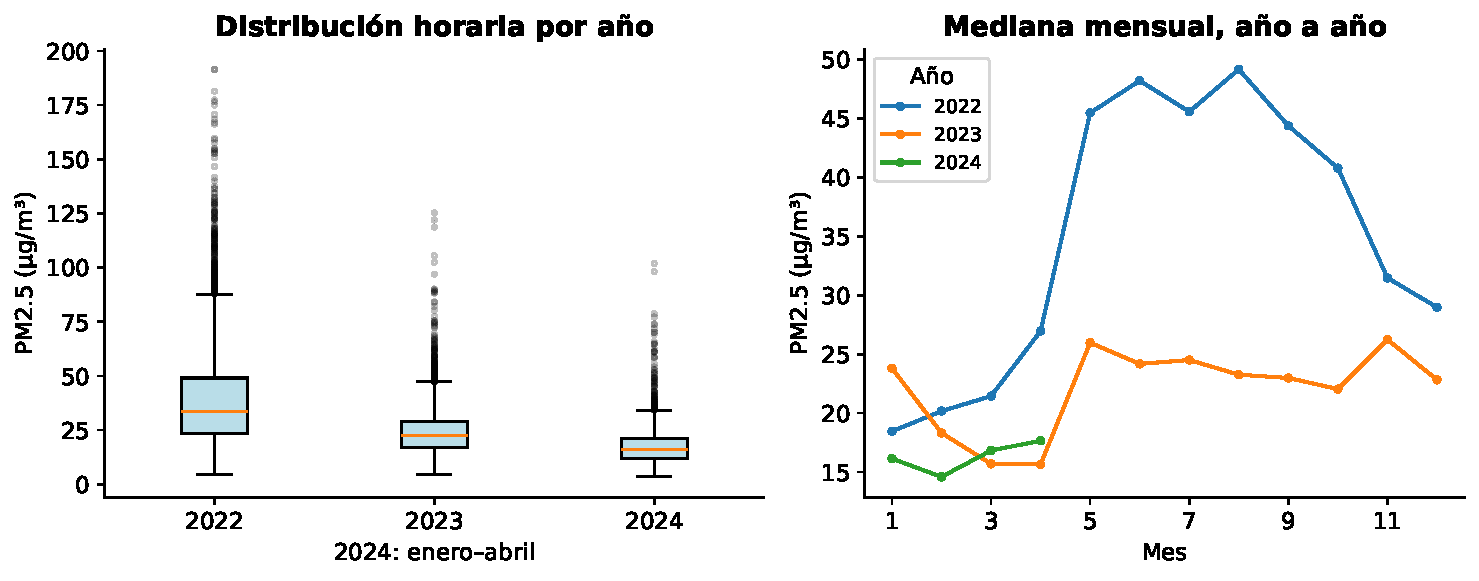
\includegraphics[width=\columnwidth]{figures/12_distribucion_anual.pdf}
\caption{Cambio de nivel entre años y comparación de medianas mensuales.}
\label{fig:regimen}
\end{figure}

\subsection{Dependencia temporal}
\label{sec:autocorrelacion}

Entre horas consecutivas la correlación de Pearson es de 0,912 (19.343 pares completos). La autocorrelación cae a 0,464 en el rezago 12 y vuelve a subir a 0,651 en el rezago 24, lo que muestra el ciclo diario. La autocorrelación parcial se concentra en el primer rezago (0,912), es negativa en el segundo ($-0{,}184$) y no supera 0,12 en valor absoluto entre los rezagos 3 y 24 (Fig.~\ref{fig:acf}). Los rezagos inmediatos aportan la información propia de corto plazo, mientras que el repunte a 24 horas corresponde al ciclo diario y puede representarse con variables de calendario en lugar de decenas de rezagos. Cuál de las dos opciones rinde más se responde comparando modelos con y sin calendario (PI2).

\begin{figure}[t]
\centering
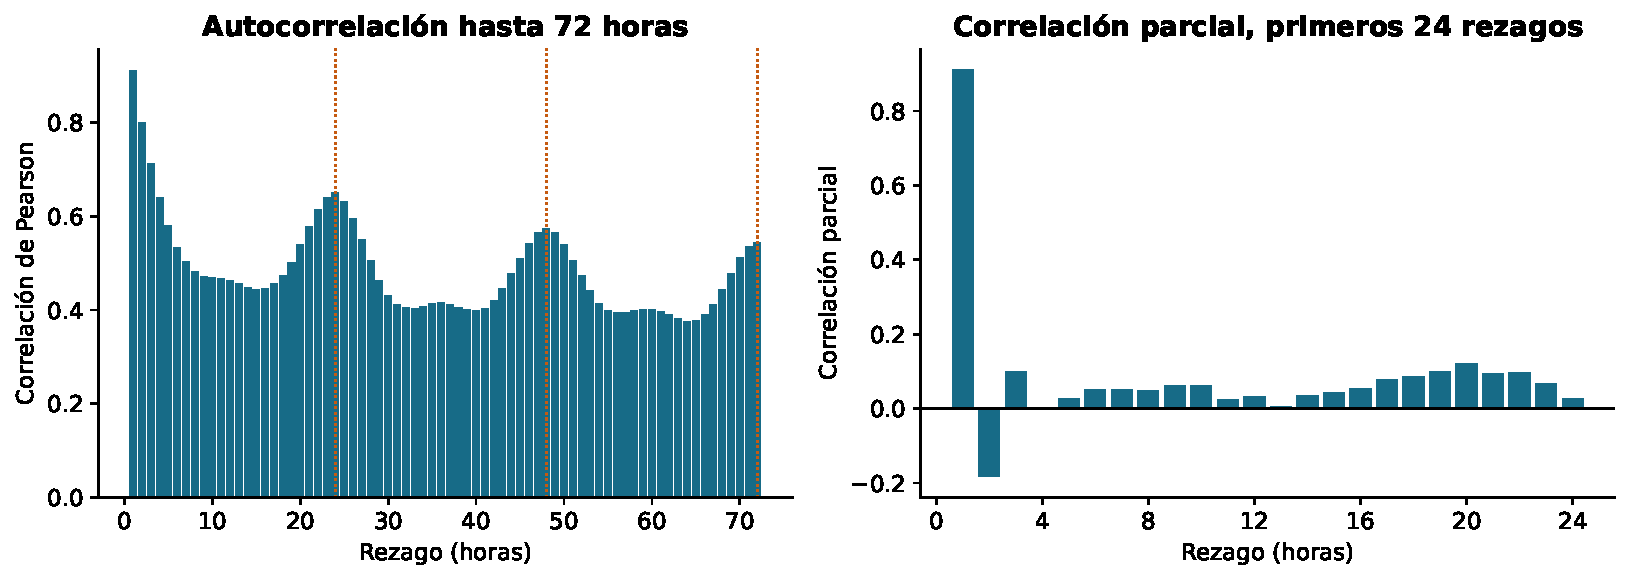
\includegraphics[width=\columnwidth]{figures/13_autocorrelacion.pdf}
\caption{Autocorrelación y autocorrelación parcial de PM2.5 hasta 48 horas, calculadas con las horas en que ambos valores están disponibles.}
\label{fig:acf}
\end{figure}

\subsection{Implicaciones para el modelado}
\label{sec:implicaciones}

El análisis exploratorio condiciona el diseño de la segunda etapa en cuatro puntos: los faltantes se agrupan en tramos y no se imputan, por lo que cada hora utilizable exige respuesta e historial completos; los valores extremos se conservan; la partición debe ser cronológica y sus métricas desagregadas por bloque, por el cambio de régimen; y el baseline natural es la persistencia, dada la correlación de 0,912 a una hora. Estas decisiones se concretan en la sección~\ref{sec:preproc}.
 después de ellas.
% Figuras esperadas en figures/ (las mismas de la notebook 01_eda).

\subsection{Calidad de los datos y valores faltantes}
\label{sec:faltantes}

De las 20.424 horas del periodo, 1.033 (5,06~\%) no tienen medición de PM2.5. Esa cifra agregada describe mal el problema: las ausencias se agrupan en 47 interrupciones con una mediana de 11 horas, y las 12 que duran 24 horas o más concentran 700 horas, el 68~\% de todos los faltantes (la mayor dura 126 horas). El archivo no documenta la causa, por lo que no puede asumirse que los faltantes sean aleatorios. Si coincidieran con episodios de alta concentración, los estadísticos descriptivos subestimarían los valores extremos. Por eso no se imputa ni se interpola ningún valor: las horas sin medición se conservan explícitamente en la serie.

Se aplicaron tres controles de coherencia. Ninguna de las 18.671 horas con PM2.5 y PM10 simultáneos presenta PM2.5 por encima de PM10, la racha máxima de valores idénticos consecutivos es de 2 (descarta un sensor bloqueado) y se observaron 49 variaciones horarias superiores a 50~\textmu g/m\textsuperscript{3}, con un máximo de 121,0. Estas últimas se señalan para revisión, pero no se descartan.

\subsection{Distribución y valores extremos}
\label{sec:distribucion}

La serie disponible (19.391 mediciones) tiene media de 29,29 y mediana de 24,50~\textmu g/m\textsuperscript{3}, desviación estándar de 18,17, percentil 95 de 65,31 y máximo de 191,5. La asimetría es de 2,11: una minoría de horas con concentraciones altas arrastra el promedio. Al ser la variable objetivo continua, no existe un desbalance de clases en sentido estricto, pero la distribución produce un efecto equivalente, porque las concentraciones altas están poco representadas.

La regla de 1,5 veces el rango intercuartílico señala 1.126 mediciones (5,81~\%). No se eliminan: el 95~\% corresponde a 2022, se concentran entre mayo y octubre y entre las 12:00 y las 16:00, que es la franja de mayor mediana horaria. Un error instrumental no reproduciría esa estructura estacional y horaria, de modo que la evidencia favorece interpretarlas como episodios reales de contaminación, que además son las horas de mayor relevancia sanitaria. Como contexto, de los 795 días con al menos 18 horas medidas, el 93~\% supera la guía diaria de la OMS (15~\textmu g/m\textsuperscript{3}) y el 10,3~\% el estándar peruano (50~\textmu g/m\textsuperscript{3}).

\subsection{Patrón diario y cambio de régimen}
\label{sec:regimen}

La mediana horaria alcanza su máximo a las 14:00 (34,4~\textmu g/m\textsuperscript{3}) y su mínimo a las 22:00 (17,0), por lo que la hora del día está asociada al nivel de PM2.5. Esta es una diferencia descriptiva; que mejore la predicción debe comprobarse con modelos.

El nivel medio desciende a lo largo del periodo: 38,8~\textmu g/m\textsuperscript{3} en 2022, 23,8 en 2023 y 17,7 en enero–abril de 2024. Parte de la caída de 2024 es estacional, pero 2022 supera a 2023 en 11 de los 12 meses, con una diferencia concentrada entre mayo y octubre, de modo que el calendario no la explica por completo (Fig.~\ref{fig:regimen}). Una partición cronológica entrena entonces en un régimen de concentraciones más altas que el de evaluación, y el error absoluto no es comparable entre tramos; las métricas deberán reportarse por separado para cada bloque.

\begin{figure}[t]
\centering
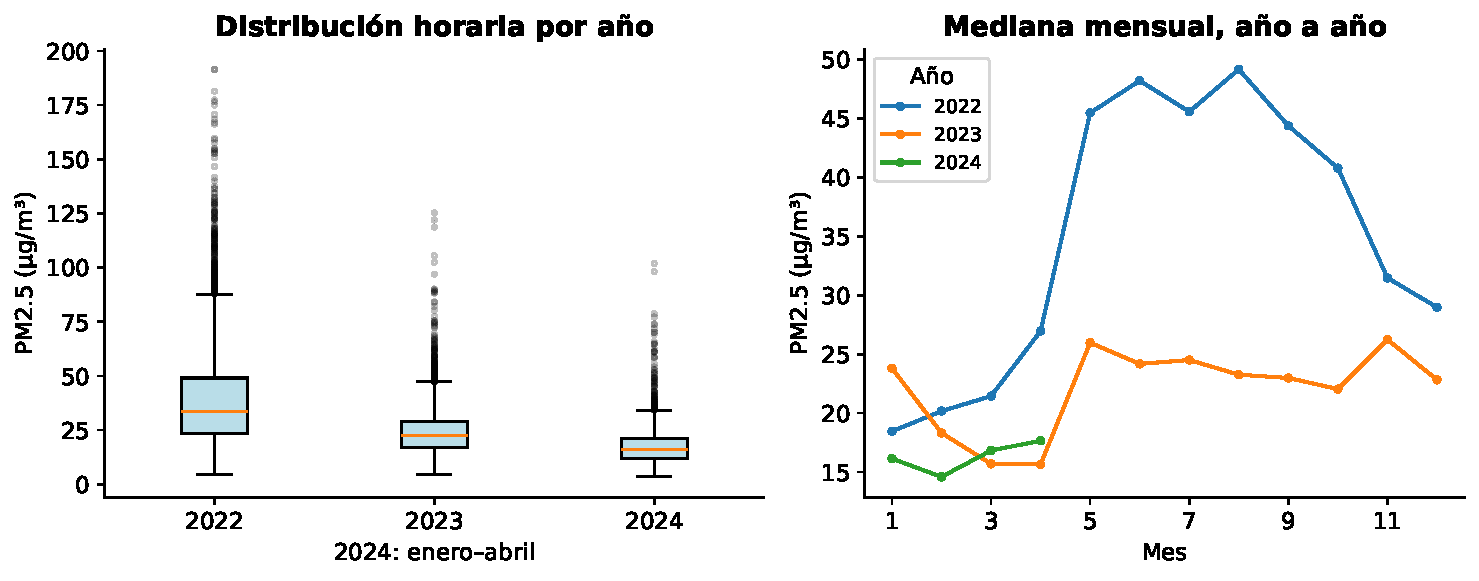
\includegraphics[width=\columnwidth]{figures/12_distribucion_anual.pdf}
\caption{Cambio de nivel entre años y comparación de medianas mensuales.}
\label{fig:regimen}
\end{figure}

\subsection{Dependencia temporal}
\label{sec:autocorrelacion}

Entre horas consecutivas la correlación de Pearson es de 0,912 (19.343 pares completos). La autocorrelación cae a 0,464 en el rezago 12 y vuelve a subir a 0,651 en el rezago 24, lo que muestra el ciclo diario. La autocorrelación parcial se concentra en el primer rezago (0,912), es negativa en el segundo ($-0{,}184$) y no supera 0,12 en valor absoluto entre los rezagos 3 y 24 (Fig.~\ref{fig:acf}). Los rezagos inmediatos aportan la información propia de corto plazo, mientras que el repunte a 24 horas corresponde al ciclo diario y puede representarse con variables de calendario en lugar de decenas de rezagos. Cuál de las dos opciones rinde más se responde comparando modelos con y sin calendario (PI2).

\begin{figure}[t]
\centering
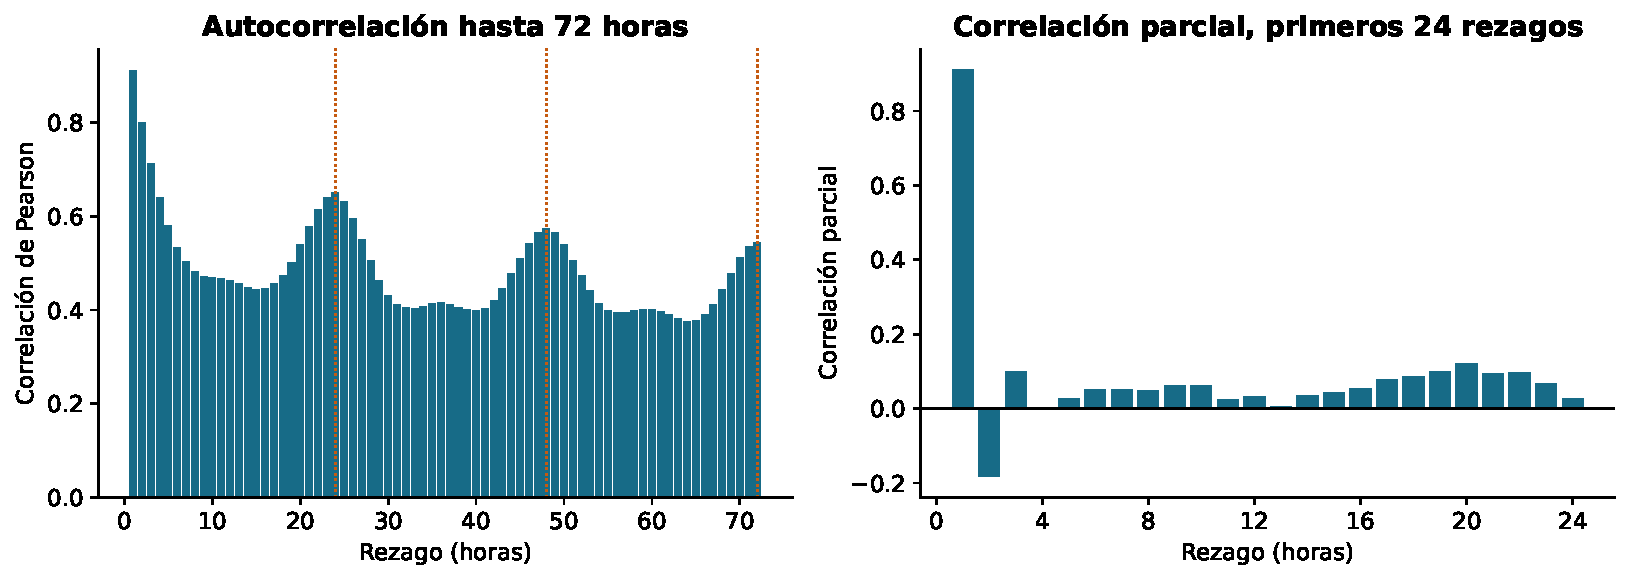
\includegraphics[width=\columnwidth]{figures/13_autocorrelacion.pdf}
\caption{Autocorrelación y autocorrelación parcial de PM2.5 hasta 48 horas, calculadas con las horas en que ambos valores están disponibles.}
\label{fig:acf}
\end{figure}

\subsection{Implicaciones para el modelado}
\label{sec:implicaciones}

El análisis exploratorio condiciona el diseño de la segunda etapa en cuatro puntos: los faltantes se agrupan en tramos y no se imputan, por lo que cada hora utilizable exige respuesta e historial completos; los valores extremos se conservan; la partición debe ser cronológica y sus métricas desagregadas por bloque, por el cambio de régimen; y el baseline natural es la persistencia, dada la correlación de 0,912 a una hora. Estas decisiones se concretan en la sección~\ref{sec:preproc}.


% Sección 4: preprocesamiento e ingeniería de características (Rol 1, P2).
% Se inserta con % Sección 4: preprocesamiento e ingeniería de características (Rol 1, P2).
% Se inserta con % Sección 4: preprocesamiento e ingeniería de características (Rol 1, P2).
% Se inserta con \input{seccion_4_preprocesamiento}. Requiere booktabs.
% Figura: figures/14_particiones_cronologicas.pdf (scripts/03_figura_particiones.py).
% Las cifras provienen de data/processed/*.csv (scripts/01 y 02).

\section{Preprocesamiento e ingeniería de características}
\label{sec:preproc}

\subsection{Conjunto supervisado y variable objetivo}

Cada ejemplo corresponde a un instante $t$ en que se hace el pronóstico. La respuesta es $y_t=\mathrm{PM}_{2{,}5}(t+1)$, la concentración exactamente una hora después, y las entradas usan únicamente mediciones en $t$ o antes. Como la rejilla horaria se conserva completa, el desplazamiento corresponde siempre a una hora real y no al siguiente registro disponible. El valor actual $\mathrm{PM}_{2{,}5}(t)$ es además el pronóstico del baseline de persistencia, por lo que se incluye como entrada.

\subsection{Variables de entrada}

La Tabla~\ref{tab:vars} resume las 11 variables. Los rezagos de 1, 3 y 6 horas capturan la dependencia inmediata observada en la autocorrelación parcial; los de 12 y 24 horas recogen el ciclo diario; y las medias móviles de 3, 6 y 24 horas, que incluyen el instante $t$, resumen el nivel reciente con menor ruido que un valor aislado. Todas se calculan con desplazamientos hacia atrás o ventanas finales, de modo que ninguna contiene información posterior a $t$. Las medias móviles exigen la ventana completa; con un hueco, la fila se descarta.

\begin{table}[t]
\centering
\caption{Variables del conjunto supervisado.}
\label{tab:vars}
\small
\begin{tabular}{@{}p{3.45cm}p{3.95cm}@{}}
\toprule
Variable & Definición \\
\midrule
\texttt{pm25\_t} & $\mathrm{PM}_{2{,}5}(t)$ \\
\texttt{pm25\_lag$k$} & $\mathrm{PM}_{2{,}5}(t-k)$, $k\in\{1,3,6,12,24\}$ h \\
\texttt{pm25\_media$w$h} & media de las últimas $w\in\{3,6,24\}$ h, incluida $t$ \\
\texttt{hora\_objetivo} & hora del día de $t+1$ (0--23) \\
\texttt{dia\_semana\_objetivo} & día de la semana de $t+1$ (0 = lunes) \\
\midrule
\texttt{y\_pm25\_t1} & respuesta: $\mathrm{PM}_{2{,}5}(t+1)$ \\
\bottomrule
\end{tabular}
\end{table}

La hora y el día corresponden a $t+1$, el instante que se pronostica, que se conoce de antemano. Se codifican dentro del pipeline: la hora con seno y coseno, para que las 23:00 y las 00:00 resulten vecinas, y el día de la semana con variables indicadoras, porque el efecto de fin de semana no sigue una senoide. El conjunto sin calendario usa solo las nueve variables de historial, con los mismos ejemplos, lo que permite comparar ambos enfoques en igualdad de condiciones.

\subsection{Faltantes y ventanas incompletas}

No se imputan valores, ni con ceros ni por interpolación. Un instante es utilizable solo si tiene la respuesta y todo su historial; en caso contrario se descarta. De los 20.424 instantes de la rejilla quedan 18.276 (89,5~\%) (Tabla~\ref{tab:perdida}). Los descartes se deben a que 1.034 instantes no tienen respuesta, 1.033 no tienen medición actual, 1.967 tienen algún rezago faltante y 2.060 una media móvil incompleta (las causas se solapan). Como las interrupciones son largas, un solo hueco invalida muchas filas vecinas. Todos los modelos y el baseline se evalúan sobre estas mismas filas, para que las comparaciones no dependan de diferencias de muestra.

\begin{table}[t]
\centering
\caption{Filas descartadas por faltantes (las causas pueden coincidir).}
\label{tab:perdida}
\small
\begin{tabular}{@{}lrr@{}}
\toprule
Concepto & Filas & \% rejilla \\
\midrule
Instantes $t$ en la rejilla & 20.424 & 100,0 \\
Sin respuesta $\mathrm{PM}_{2{,}5}(t+1)$ & 1.034 & 5,1 \\
Sin medición actual & 1.033 & 5,1 \\
Algún rezago faltante & 1.967 & 9,6 \\
Alguna media móvil incompleta & 2.060 & 10,1 \\
\midrule
\textbf{Filas utilizables} & \textbf{18.276} & \textbf{89,5} \\
\bottomrule
\end{tabular}
\end{table}

\subsection{Partición cronológica}

Los datos se dividen en tres bloques contiguos y disjuntos, sin barajar filas: entrenamiento (enero de 2022 a junio de 2023), validación (julio a diciembre de 2023) y prueba (enero a abril de 2024). La partición se asigna según el instante de la respuesta $t+1$, de modo que ninguna etiqueta de entrenamiento cae en el periodo de validación ni una de validación en el de prueba. Una fila de validación sí puede usar como entrada observaciones del periodo de entrenamiento, algo legítimo porque son pasadas. Los cortes se fijaron antes de ver resultados de ningún modelo. El ajuste de hiperparámetros se hará con validación de origen móvil dentro del entrenamiento, nunca con particiones aleatorias.

\begin{table}[t]
\centering
\caption{Conjunto supervisado por bloque (respuesta en \textmu g/m\textsuperscript{3}).}
\label{tab:part}
\small
\begin{tabular}{@{}lrrrrr@{}}
\toprule
Bloque & Filas & Media & Mediana & P95 & Máx. \\
\midrule
Entrenamiento & 11.551 & 32,9 & 27,8 & 72,2 & 191,5 \\
Validación & 4.024 & 25,1 & 23,7 & 41,8 & 125,3 \\
Prueba & 2.701 & 17,8 & 16,1 & 32,2 & 101,9 \\
\bottomrule
\end{tabular}
\end{table}

La Tabla~\ref{tab:part} y la Fig.~\ref{fig:part} muestran que la distribución de la respuesta cambia entre bloques: la media baja de 32,9 a 17,8 y el máximo de 191,5 a 101,9. El modelo se entrena, por tanto, en un régimen de concentraciones más altas del que se evalúa. Esto obliga a reportar las métricas por bloque y a comparar cada modelo con la persistencia calculada sobre el mismo bloque, ya que un mismo error absoluto no significa el mismo desempeño relativo en cada tramo.

\begin{figure}[t]
\centering
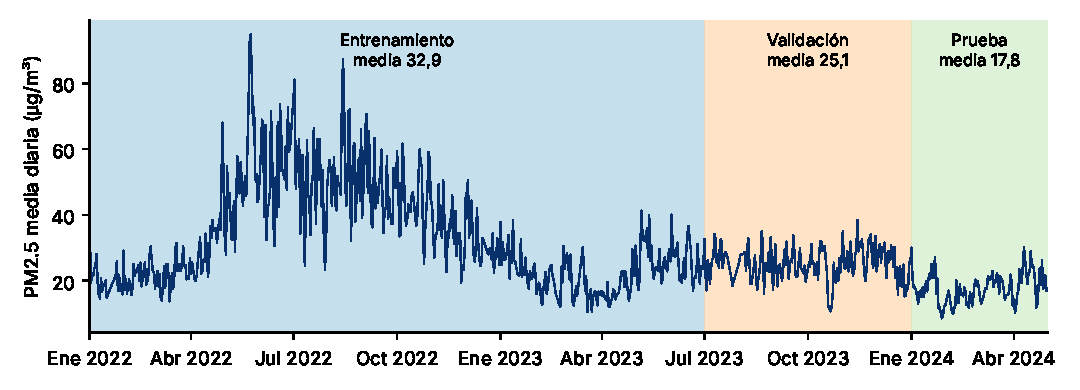
\includegraphics[width=\columnwidth]{figures/14_particiones_cronologicas.pdf}
\caption{Partición cronológica sobre la media diaria de PM2.5 (días con al menos 18 horas medidas). Se indica la media de la respuesta de cada bloque.}
\label{fig:part}
\end{figure}

\subsection{Preprocesamiento dentro del pipeline y prevención de fuga}

La fuga de información, es decir, que el modelo use durante el entrenamiento datos que no estarían disponibles al predecir, es una causa conocida de resultados optimistas~\cite{kaufman2012}. Para evitarla, el escalado se ejecuta dentro de un \texttt{Pipeline} de scikit-learn: las nueve variables de historial se estandarizan con la media y la desviación del entrenamiento, y esos parámetros se aplican sin reajuste a validación y prueba. Ajustar el escalador con todos los datos filtraría información de los bloques posteriores: la media de $\mathrm{PM}_{2{,}5}(t)$ es de 32,94 en entrenamiento y de 28,98 en el conjunto completo.

La ausencia de fuga se comprueba de forma explícita con un guion reproducible (\texttt{scripts/02\_verificar\_fuga.py}) que ejecuta 12 verificaciones, todas superadas (Tabla~\ref{tab:fuga}). La prueba central altera por completo los valores posteriores a un instante de corte y comprueba que las entradas en ese instante no cambian. Como control negativo, se añade a propósito una variable con información futura y se confirma que la prueba la detecta.

\begin{table}[t]
\centering
\caption{Comprobaciones de ausencia de fuga de información.}
\label{tab:fuga}
\small
\begin{tabular}{@{}p{5.9cm}c@{}}
\toprule
Comprobación & Resultado \\
\midrule
Recálculo independiente con solo el pasado (500 filas) & Superada \\
Las entradas no cambian si se altera el futuro (8 cortes) & Superada \\
Respuesta igual a $\mathrm{PM}_{2{,}5}(t+1)$ y calendario de $t+1$ & Superada \\
Bloques ordenados, disjuntos y completos & Superada \\
Filas con hueco excluidas, sin ceros inventados & Superada \\
Escalador ajustado solo con entrenamiento (con y sin calendario) & Superada \\
Control negativo: una fuga deliberada es detectada & Superada \\
\bottomrule
\end{tabular}
\end{table}
. Requiere booktabs.
% Figura: figures/14_particiones_cronologicas.pdf (scripts/03_figura_particiones.py).
% Las cifras provienen de data/processed/*.csv (scripts/01 y 02).

\section{Preprocesamiento e ingeniería de características}
\label{sec:preproc}

\subsection{Conjunto supervisado y variable objetivo}

Cada ejemplo corresponde a un instante $t$ en que se hace el pronóstico. La respuesta es $y_t=\mathrm{PM}_{2{,}5}(t+1)$, la concentración exactamente una hora después, y las entradas usan únicamente mediciones en $t$ o antes. Como la rejilla horaria se conserva completa, el desplazamiento corresponde siempre a una hora real y no al siguiente registro disponible. El valor actual $\mathrm{PM}_{2{,}5}(t)$ es además el pronóstico del baseline de persistencia, por lo que se incluye como entrada.

\subsection{Variables de entrada}

La Tabla~\ref{tab:vars} resume las 11 variables. Los rezagos de 1, 3 y 6 horas capturan la dependencia inmediata observada en la autocorrelación parcial; los de 12 y 24 horas recogen el ciclo diario; y las medias móviles de 3, 6 y 24 horas, que incluyen el instante $t$, resumen el nivel reciente con menor ruido que un valor aislado. Todas se calculan con desplazamientos hacia atrás o ventanas finales, de modo que ninguna contiene información posterior a $t$. Las medias móviles exigen la ventana completa; con un hueco, la fila se descarta.

\begin{table}[t]
\centering
\caption{Variables del conjunto supervisado.}
\label{tab:vars}
\small
\begin{tabular}{@{}p{3.45cm}p{3.95cm}@{}}
\toprule
Variable & Definición \\
\midrule
\texttt{pm25\_t} & $\mathrm{PM}_{2{,}5}(t)$ \\
\texttt{pm25\_lag$k$} & $\mathrm{PM}_{2{,}5}(t-k)$, $k\in\{1,3,6,12,24\}$ h \\
\texttt{pm25\_media$w$h} & media de las últimas $w\in\{3,6,24\}$ h, incluida $t$ \\
\texttt{hora\_objetivo} & hora del día de $t+1$ (0--23) \\
\texttt{dia\_semana\_objetivo} & día de la semana de $t+1$ (0 = lunes) \\
\midrule
\texttt{y\_pm25\_t1} & respuesta: $\mathrm{PM}_{2{,}5}(t+1)$ \\
\bottomrule
\end{tabular}
\end{table}

La hora y el día corresponden a $t+1$, el instante que se pronostica, que se conoce de antemano. Se codifican dentro del pipeline: la hora con seno y coseno, para que las 23:00 y las 00:00 resulten vecinas, y el día de la semana con variables indicadoras, porque el efecto de fin de semana no sigue una senoide. El conjunto sin calendario usa solo las nueve variables de historial, con los mismos ejemplos, lo que permite comparar ambos enfoques en igualdad de condiciones.

\subsection{Faltantes y ventanas incompletas}

No se imputan valores, ni con ceros ni por interpolación. Un instante es utilizable solo si tiene la respuesta y todo su historial; en caso contrario se descarta. De los 20.424 instantes de la rejilla quedan 18.276 (89,5~\%) (Tabla~\ref{tab:perdida}). Los descartes se deben a que 1.034 instantes no tienen respuesta, 1.033 no tienen medición actual, 1.967 tienen algún rezago faltante y 2.060 una media móvil incompleta (las causas se solapan). Como las interrupciones son largas, un solo hueco invalida muchas filas vecinas. Todos los modelos y el baseline se evalúan sobre estas mismas filas, para que las comparaciones no dependan de diferencias de muestra.

\begin{table}[t]
\centering
\caption{Filas descartadas por faltantes (las causas pueden coincidir).}
\label{tab:perdida}
\small
\begin{tabular}{@{}lrr@{}}
\toprule
Concepto & Filas & \% rejilla \\
\midrule
Instantes $t$ en la rejilla & 20.424 & 100,0 \\
Sin respuesta $\mathrm{PM}_{2{,}5}(t+1)$ & 1.034 & 5,1 \\
Sin medición actual & 1.033 & 5,1 \\
Algún rezago faltante & 1.967 & 9,6 \\
Alguna media móvil incompleta & 2.060 & 10,1 \\
\midrule
\textbf{Filas utilizables} & \textbf{18.276} & \textbf{89,5} \\
\bottomrule
\end{tabular}
\end{table}

\subsection{Partición cronológica}

Los datos se dividen en tres bloques contiguos y disjuntos, sin barajar filas: entrenamiento (enero de 2022 a junio de 2023), validación (julio a diciembre de 2023) y prueba (enero a abril de 2024). La partición se asigna según el instante de la respuesta $t+1$, de modo que ninguna etiqueta de entrenamiento cae en el periodo de validación ni una de validación en el de prueba. Una fila de validación sí puede usar como entrada observaciones del periodo de entrenamiento, algo legítimo porque son pasadas. Los cortes se fijaron antes de ver resultados de ningún modelo. El ajuste de hiperparámetros se hará con validación de origen móvil dentro del entrenamiento, nunca con particiones aleatorias.

\begin{table}[t]
\centering
\caption{Conjunto supervisado por bloque (respuesta en \textmu g/m\textsuperscript{3}).}
\label{tab:part}
\small
\begin{tabular}{@{}lrrrrr@{}}
\toprule
Bloque & Filas & Media & Mediana & P95 & Máx. \\
\midrule
Entrenamiento & 11.551 & 32,9 & 27,8 & 72,2 & 191,5 \\
Validación & 4.024 & 25,1 & 23,7 & 41,8 & 125,3 \\
Prueba & 2.701 & 17,8 & 16,1 & 32,2 & 101,9 \\
\bottomrule
\end{tabular}
\end{table}

La Tabla~\ref{tab:part} y la Fig.~\ref{fig:part} muestran que la distribución de la respuesta cambia entre bloques: la media baja de 32,9 a 17,8 y el máximo de 191,5 a 101,9. El modelo se entrena, por tanto, en un régimen de concentraciones más altas del que se evalúa. Esto obliga a reportar las métricas por bloque y a comparar cada modelo con la persistencia calculada sobre el mismo bloque, ya que un mismo error absoluto no significa el mismo desempeño relativo en cada tramo.

\begin{figure}[t]
\centering
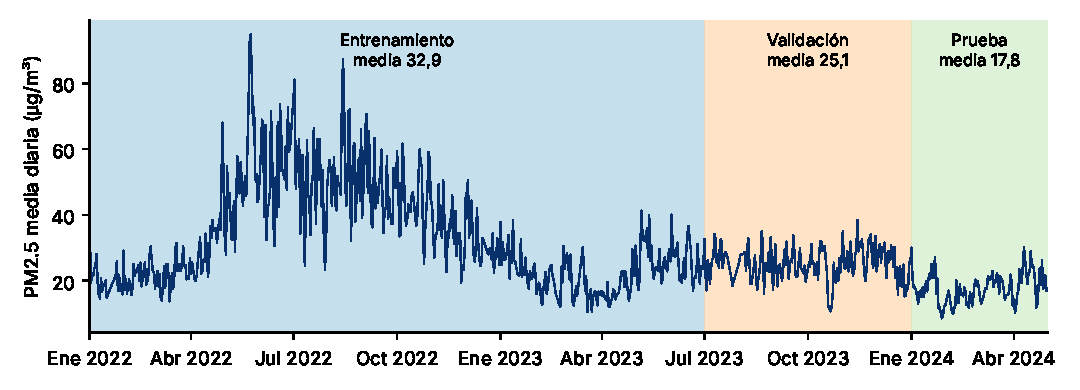
\includegraphics[width=\columnwidth]{figures/14_particiones_cronologicas.pdf}
\caption{Partición cronológica sobre la media diaria de PM2.5 (días con al menos 18 horas medidas). Se indica la media de la respuesta de cada bloque.}
\label{fig:part}
\end{figure}

\subsection{Preprocesamiento dentro del pipeline y prevención de fuga}

La fuga de información, es decir, que el modelo use durante el entrenamiento datos que no estarían disponibles al predecir, es una causa conocida de resultados optimistas~\cite{kaufman2012}. Para evitarla, el escalado se ejecuta dentro de un \texttt{Pipeline} de scikit-learn: las nueve variables de historial se estandarizan con la media y la desviación del entrenamiento, y esos parámetros se aplican sin reajuste a validación y prueba. Ajustar el escalador con todos los datos filtraría información de los bloques posteriores: la media de $\mathrm{PM}_{2{,}5}(t)$ es de 32,94 en entrenamiento y de 28,98 en el conjunto completo.

La ausencia de fuga se comprueba de forma explícita con un guion reproducible (\texttt{scripts/02\_verificar\_fuga.py}) que ejecuta 12 verificaciones, todas superadas (Tabla~\ref{tab:fuga}). La prueba central altera por completo los valores posteriores a un instante de corte y comprueba que las entradas en ese instante no cambian. Como control negativo, se añade a propósito una variable con información futura y se confirma que la prueba la detecta.

\begin{table}[t]
\centering
\caption{Comprobaciones de ausencia de fuga de información.}
\label{tab:fuga}
\small
\begin{tabular}{@{}p{5.9cm}c@{}}
\toprule
Comprobación & Resultado \\
\midrule
Recálculo independiente con solo el pasado (500 filas) & Superada \\
Las entradas no cambian si se altera el futuro (8 cortes) & Superada \\
Respuesta igual a $\mathrm{PM}_{2{,}5}(t+1)$ y calendario de $t+1$ & Superada \\
Bloques ordenados, disjuntos y completos & Superada \\
Filas con hueco excluidas, sin ceros inventados & Superada \\
Escalador ajustado solo con entrenamiento (con y sin calendario) & Superada \\
Control negativo: una fuga deliberada es detectada & Superada \\
\bottomrule
\end{tabular}
\end{table}
. Requiere booktabs.
% Figura: figures/14_particiones_cronologicas.pdf (scripts/03_figura_particiones.py).
% Las cifras provienen de data/processed/*.csv (scripts/01 y 02).

\section{Preprocesamiento e ingeniería de características}
\label{sec:preproc}

\subsection{Conjunto supervisado y variable objetivo}

Cada ejemplo corresponde a un instante $t$ en que se hace el pronóstico. La respuesta es $y_t=\mathrm{PM}_{2{,}5}(t+1)$, la concentración exactamente una hora después, y las entradas usan únicamente mediciones en $t$ o antes. Como la rejilla horaria se conserva completa, el desplazamiento corresponde siempre a una hora real y no al siguiente registro disponible. El valor actual $\mathrm{PM}_{2{,}5}(t)$ es además el pronóstico del baseline de persistencia, por lo que se incluye como entrada.

\subsection{Variables de entrada}

La Tabla~\ref{tab:vars} resume las 11 variables. Los rezagos de 1, 3 y 6 horas capturan la dependencia inmediata observada en la autocorrelación parcial; los de 12 y 24 horas recogen el ciclo diario; y las medias móviles de 3, 6 y 24 horas, que incluyen el instante $t$, resumen el nivel reciente con menor ruido que un valor aislado. Todas se calculan con desplazamientos hacia atrás o ventanas finales, de modo que ninguna contiene información posterior a $t$. Las medias móviles exigen la ventana completa; con un hueco, la fila se descarta.

\begin{table}[t]
\centering
\caption{Variables del conjunto supervisado.}
\label{tab:vars}
\small
\begin{tabular}{@{}p{3.45cm}p{3.95cm}@{}}
\toprule
Variable & Definición \\
\midrule
\texttt{pm25\_t} & $\mathrm{PM}_{2{,}5}(t)$ \\
\texttt{pm25\_lag$k$} & $\mathrm{PM}_{2{,}5}(t-k)$, $k\in\{1,3,6,12,24\}$ h \\
\texttt{pm25\_media$w$h} & media de las últimas $w\in\{3,6,24\}$ h, incluida $t$ \\
\texttt{hora\_objetivo} & hora del día de $t+1$ (0--23) \\
\texttt{dia\_semana\_objetivo} & día de la semana de $t+1$ (0 = lunes) \\
\midrule
\texttt{y\_pm25\_t1} & respuesta: $\mathrm{PM}_{2{,}5}(t+1)$ \\
\bottomrule
\end{tabular}
\end{table}

La hora y el día corresponden a $t+1$, el instante que se pronostica, que se conoce de antemano. Se codifican dentro del pipeline: la hora con seno y coseno, para que las 23:00 y las 00:00 resulten vecinas, y el día de la semana con variables indicadoras, porque el efecto de fin de semana no sigue una senoide. El conjunto sin calendario usa solo las nueve variables de historial, con los mismos ejemplos, lo que permite comparar ambos enfoques en igualdad de condiciones.

\subsection{Faltantes y ventanas incompletas}

No se imputan valores, ni con ceros ni por interpolación. Un instante es utilizable solo si tiene la respuesta y todo su historial; en caso contrario se descarta. De los 20.424 instantes de la rejilla quedan 18.276 (89,5~\%) (Tabla~\ref{tab:perdida}). Los descartes se deben a que 1.034 instantes no tienen respuesta, 1.033 no tienen medición actual, 1.967 tienen algún rezago faltante y 2.060 una media móvil incompleta (las causas se solapan). Como las interrupciones son largas, un solo hueco invalida muchas filas vecinas. Todos los modelos y el baseline se evalúan sobre estas mismas filas, para que las comparaciones no dependan de diferencias de muestra.

\begin{table}[t]
\centering
\caption{Filas descartadas por faltantes (las causas pueden coincidir).}
\label{tab:perdida}
\small
\begin{tabular}{@{}lrr@{}}
\toprule
Concepto & Filas & \% rejilla \\
\midrule
Instantes $t$ en la rejilla & 20.424 & 100,0 \\
Sin respuesta $\mathrm{PM}_{2{,}5}(t+1)$ & 1.034 & 5,1 \\
Sin medición actual & 1.033 & 5,1 \\
Algún rezago faltante & 1.967 & 9,6 \\
Alguna media móvil incompleta & 2.060 & 10,1 \\
\midrule
\textbf{Filas utilizables} & \textbf{18.276} & \textbf{89,5} \\
\bottomrule
\end{tabular}
\end{table}

\subsection{Partición cronológica}

Los datos se dividen en tres bloques contiguos y disjuntos, sin barajar filas: entrenamiento (enero de 2022 a junio de 2023), validación (julio a diciembre de 2023) y prueba (enero a abril de 2024). La partición se asigna según el instante de la respuesta $t+1$, de modo que ninguna etiqueta de entrenamiento cae en el periodo de validación ni una de validación en el de prueba. Una fila de validación sí puede usar como entrada observaciones del periodo de entrenamiento, algo legítimo porque son pasadas. Los cortes se fijaron antes de ver resultados de ningún modelo. El ajuste de hiperparámetros se hará con validación de origen móvil dentro del entrenamiento, nunca con particiones aleatorias.

\begin{table}[t]
\centering
\caption{Conjunto supervisado por bloque (respuesta en \textmu g/m\textsuperscript{3}).}
\label{tab:part}
\small
\begin{tabular}{@{}lrrrrr@{}}
\toprule
Bloque & Filas & Media & Mediana & P95 & Máx. \\
\midrule
Entrenamiento & 11.551 & 32,9 & 27,8 & 72,2 & 191,5 \\
Validación & 4.024 & 25,1 & 23,7 & 41,8 & 125,3 \\
Prueba & 2.701 & 17,8 & 16,1 & 32,2 & 101,9 \\
\bottomrule
\end{tabular}
\end{table}

La Tabla~\ref{tab:part} y la Fig.~\ref{fig:part} muestran que la distribución de la respuesta cambia entre bloques: la media baja de 32,9 a 17,8 y el máximo de 191,5 a 101,9. El modelo se entrena, por tanto, en un régimen de concentraciones más altas del que se evalúa. Esto obliga a reportar las métricas por bloque y a comparar cada modelo con la persistencia calculada sobre el mismo bloque, ya que un mismo error absoluto no significa el mismo desempeño relativo en cada tramo.

\begin{figure}[t]
\centering
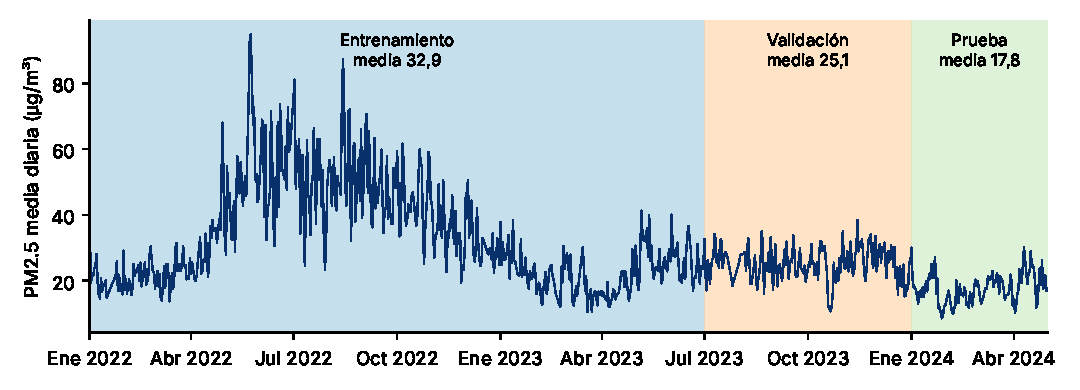
\includegraphics[width=\columnwidth]{figures/14_particiones_cronologicas.pdf}
\caption{Partición cronológica sobre la media diaria de PM2.5 (días con al menos 18 horas medidas). Se indica la media de la respuesta de cada bloque.}
\label{fig:part}
\end{figure}

\subsection{Preprocesamiento dentro del pipeline y prevención de fuga}

La fuga de información, es decir, que el modelo use durante el entrenamiento datos que no estarían disponibles al predecir, es una causa conocida de resultados optimistas~\cite{kaufman2012}. Para evitarla, el escalado se ejecuta dentro de un \texttt{Pipeline} de scikit-learn: las nueve variables de historial se estandarizan con la media y la desviación del entrenamiento, y esos parámetros se aplican sin reajuste a validación y prueba. Ajustar el escalador con todos los datos filtraría información de los bloques posteriores: la media de $\mathrm{PM}_{2{,}5}(t)$ es de 32,94 en entrenamiento y de 28,98 en el conjunto completo.

La ausencia de fuga se comprueba de forma explícita con un guion reproducible (\texttt{scripts/02\_verificar\_fuga.py}) que ejecuta 12 verificaciones, todas superadas (Tabla~\ref{tab:fuga}). La prueba central altera por completo los valores posteriores a un instante de corte y comprueba que las entradas en ese instante no cambian. Como control negativo, se añade a propósito una variable con información futura y se confirma que la prueba la detecta.

\begin{table}[t]
\centering
\caption{Comprobaciones de ausencia de fuga de información.}
\label{tab:fuga}
\small
\begin{tabular}{@{}p{5.9cm}c@{}}
\toprule
Comprobación & Resultado \\
\midrule
Recálculo independiente con solo el pasado (500 filas) & Superada \\
Las entradas no cambian si se altera el futuro (8 cortes) & Superada \\
Respuesta igual a $\mathrm{PM}_{2{,}5}(t+1)$ y calendario de $t+1$ & Superada \\
Bloques ordenados, disjuntos y completos & Superada \\
Filas con hueco excluidas, sin ceros inventados & Superada \\
Escalador ajustado solo con entrenamiento (con y sin calendario) & Superada \\
Control negativo: una fuga deliberada es detectada & Superada \\
\bottomrule
\end{tabular}
\end{table}

% A integrar en la sección 5 junto con los modelos no lineales del rol 3.
\section{Metodología y modelos}
\label{sec:metodologia}
\subsection{Baseline de persistencia}
La referencia predice la siguiente hora con la medición actual: $\hat y_t=\mathrm{PM}_{2{,}5}(t)$. No requiere ajuste y representa una referencia exigente para una serie con dependencia temporal. Se evalúa sobre las mismas filas que los modelos entrenados.

\subsection{Modelos lineales regularizados}
Ridge y Lasso predicen mediante una combinación lineal de las características de la sección~\ref{sec:preproc}. Ridge penaliza la suma de cuadrados de los coeficientes, lo que reduce su magnitud; Lasso penaliza la suma de sus valores absolutos y puede llevar algunos exactamente a cero. En ambos casos $\alpha$ controla la intensidad de regularización. Se comparan versiones con nueve variables de historial y versiones que añaden el calendario. Las nueve variables de historial se estandarizan dentro del pipeline; la hora se representa con seno y coseno y el día con indicadores, con lunes como referencia. El ajuste temporal y la selección se describen en la sección~\ref{sec:diseno}.

En validación, la persistencia obtiene MAE 3,378, RMSE 5,143, MSE 26,446 y $R^2=0{,}700$. Ridge sin calendario logra MAE 3,141 y Lasso sin calendario 3,142; con calendario alcanzan 3,205 y 3,205, respectivamente. En esta comparación el calendario no mejora el MAE, por lo que no hay evidencia de aporte en este bloque para estas variantes. Ridge sin calendario, seleccionado por MAE de validación, mejora un 7,0~\% frente a persistencia en ese bloque. En prueba alcanza MAE 2,626 frente a 2,829 de persistencia (mejora de 7,2~\%); sus RMSE son 4,766 y 5,265, respectivamente. La comparación procede de la misma muestra y no implica que el resultado se mantenga en otros periodos.

El $\alpha$ seleccionado es 0,001 para ambas variantes de Ridge y 0,01 para ambas de Lasso. El valor de Ridge está en el límite inferior de la malla, por lo que no se descarta que una regularización menor mejore la validación temporal. En Lasso sin calendario ningún coeficiente es cero; con calendario se anulan los indicadores de martes, miércoles, jueves y sábado. El coeficiente de la medición actual es positivo y el de mayor magnitud entre las variables estandarizadas del historial; los coeficientes de estas variables correlacionadas deben interpretarse conjuntamente y no como efectos causales. Los indicadores de día no están estandarizados, por lo que sus magnitudes no se comparan directamente con las del historial. Las tablas completas de métricas, búsqueda y coeficientes se encuentran en \texttt{data/processed/lineales\_*.csv}.

% Rol 3. Subsecciones a continuación de seccion_5_baseline_lineales (misma \section).
% Insertar con % Rol 3. Subsecciones a continuación de seccion_5_baseline_lineales (misma \section).
% Insertar con % Rol 3. Subsecciones a continuación de seccion_5_baseline_lineales (misma \section).
% Insertar con \input{seccion_5_no_lineales}. Requiere booktabs.
% Cifras: data/processed/no_lineales_*.csv (scripts/05_modelos_no_lineales.py).
\subsection{Modelos no lineales basados en árboles}
\label{sec:no-lineales}
Los modelos lineales suponen que cada variable aporta de forma aditiva y con el mismo coeficiente en cualquier nivel de concentración. Para relajar ese supuesto se incluyen dos conjuntos de árboles de regresión, que aprenden umbrales e interacciones (por ejemplo, entre la hora y el nivel reciente) sin especificarlos de antemano.

\textbf{Random Forest} promedia árboles profundos entrenados sobre muestras bootstrap; en cada división solo se considera una fracción aleatoria \texttt{max\_features} de las variables, lo que reduce la correlación entre árboles y, con ello, la varianza del promedio. El tamaño mínimo de hoja \texttt{min\_samples\_leaf} controla cuánto se suaviza la predicción. \textbf{HistGradientBoosting} (HistGB), la implementación de \emph{gradient boosting} de scikit-learn~\cite{pedregosa2011sklearn}, añade árboles pequeños de forma secuencial, cada uno ajustado al gradiente de la pérdida cuadrática del conjunto anterior y escalado por la tasa de aprendizaje; discretiza las variables en histogramas para acelerar la búsqueda de cortes. Es la misma familia que XGBoost y LightGBM, usada en trabajos previos con datos de SENAMHI~\cite{oblitas2024xgboost,chen2016xgboost}, y no añade dependencias al proyecto. Su parada temprana se desactiva porque separa una validación interna aleatoria, no cronológica.

Ambos modelos reciben exactamente las entradas de la sección~\ref{sec:preproc} y el mismo preprocesador que los lineales; la estandarización no altera los cortes de un árbol, pero mantenerla garantiza entradas idénticas. Se ajustan con los mismos tres cortes de origen expansivo, el mismo criterio (MAE medio de las tres ventanas) y la misma evaluación descritos en la sección~\ref{sec:diseno}, con y sin calendario y semilla fija. La Tabla~\ref{tab:mallas} resume las mallas y los valores elegidos. Las variantes con calendario obtienen menor MAE de validación cruzada (4,819 frente a 4,964 en Random Forest y 4,889 frente a 5,010 en HistGB) y también en validación, que es el criterio de selección, por lo que son las elegidas en cada familia. Los valores elegidos de \texttt{max\_features}, \texttt{min\_samples\_leaf}, \texttt{learning\_rate}, \texttt{max\_iter} y \texttt{max\_leaf\_nodes} son interiores a su malla; la malla de HistGB se amplió tras una primera búsqueda en la que \texttt{max\_iter} y \texttt{min\_samples\_leaf} quedaban en el borde. \texttt{n\_estimators} toma el mayor valor probado, pero 200 y 500 árboles difieren en menos de 0,01 de MAE, y \texttt{l2\_regularization} elige 0, es decir, sin penalización adicional. Ambos prefieren hojas grandes (20 y 100 observaciones), es decir, predicciones suavizadas.

\begin{table}[t]
\centering
\caption{Mallas de hiperparámetros y valores elegidos por MAE de validación temporal (variantes con calendario).}
\label{tab:mallas}
\small
\begin{tabular}{@{}llr@{}}
\toprule
Hiperparámetro & Valores probados & Elegido \\
\midrule
\multicolumn{3}{@{}l}{\emph{Random Forest} (30 combinaciones)} \\
\texttt{n\_estimators} & 200, 500 & 500 \\
\texttt{max\_features} & 0,33; 0,6; 1,0 & 0,6 \\
\texttt{min\_samples\_leaf} & 1, 5, 20, 50, 100 & 20 \\
\midrule
\multicolumn{3}{@{}l}{\emph{HistGB} (216 combinaciones)} \\
\texttt{learning\_rate} & 0,02; 0,05; 0,1 & 0,05 \\
\texttt{max\_iter} & 50, 100, 300, 600 & 100 \\
\texttt{max\_leaf\_nodes} & 7, 15, 31 & 15 \\
\texttt{min\_samples\_leaf} & 20, 100, 300 & 100 \\
\texttt{l2\_regularization} & 0; 1 & 0 \\
\bottomrule
\end{tabular}
\end{table}

A diferencia del rol lineal, en el que solo el mejor modelo pasó a prueba, aquí se evalúa en prueba el elegido de cada familia, para comparar familias en el periodo final. La elección de hiperparámetros, de la variante y de cada representante se hizo solo con entrenamiento y validación; prueba no se usa para escoger entre ellos. Un límite común a ambos métodos es que su predicción es un promedio de valores observados en las hojas: no pueden pronosticar concentraciones por encima de las vistas en entrenamiento y, con hojas grandes, tienden a atenuar los picos (sección~\ref{sec:regimen-alto}).
. Requiere booktabs.
% Cifras: data/processed/no_lineales_*.csv (scripts/05_modelos_no_lineales.py).
\subsection{Modelos no lineales basados en árboles}
\label{sec:no-lineales}
Los modelos lineales suponen que cada variable aporta de forma aditiva y con el mismo coeficiente en cualquier nivel de concentración. Para relajar ese supuesto se incluyen dos conjuntos de árboles de regresión, que aprenden umbrales e interacciones (por ejemplo, entre la hora y el nivel reciente) sin especificarlos de antemano.

\textbf{Random Forest} promedia árboles profundos entrenados sobre muestras bootstrap; en cada división solo se considera una fracción aleatoria \texttt{max\_features} de las variables, lo que reduce la correlación entre árboles y, con ello, la varianza del promedio. El tamaño mínimo de hoja \texttt{min\_samples\_leaf} controla cuánto se suaviza la predicción. \textbf{HistGradientBoosting} (HistGB), la implementación de \emph{gradient boosting} de scikit-learn~\cite{pedregosa2011sklearn}, añade árboles pequeños de forma secuencial, cada uno ajustado al gradiente de la pérdida cuadrática del conjunto anterior y escalado por la tasa de aprendizaje; discretiza las variables en histogramas para acelerar la búsqueda de cortes. Es la misma familia que XGBoost y LightGBM, usada en trabajos previos con datos de SENAMHI~\cite{oblitas2024xgboost,chen2016xgboost}, y no añade dependencias al proyecto. Su parada temprana se desactiva porque separa una validación interna aleatoria, no cronológica.

Ambos modelos reciben exactamente las entradas de la sección~\ref{sec:preproc} y el mismo preprocesador que los lineales; la estandarización no altera los cortes de un árbol, pero mantenerla garantiza entradas idénticas. Se ajustan con los mismos tres cortes de origen expansivo, el mismo criterio (MAE medio de las tres ventanas) y la misma evaluación descritos en la sección~\ref{sec:diseno}, con y sin calendario y semilla fija. La Tabla~\ref{tab:mallas} resume las mallas y los valores elegidos. Las variantes con calendario obtienen menor MAE de validación cruzada (4,819 frente a 4,964 en Random Forest y 4,889 frente a 5,010 en HistGB) y también en validación, que es el criterio de selección, por lo que son las elegidas en cada familia. Los valores elegidos de \texttt{max\_features}, \texttt{min\_samples\_leaf}, \texttt{learning\_rate}, \texttt{max\_iter} y \texttt{max\_leaf\_nodes} son interiores a su malla; la malla de HistGB se amplió tras una primera búsqueda en la que \texttt{max\_iter} y \texttt{min\_samples\_leaf} quedaban en el borde. \texttt{n\_estimators} toma el mayor valor probado, pero 200 y 500 árboles difieren en menos de 0,01 de MAE, y \texttt{l2\_regularization} elige 0, es decir, sin penalización adicional. Ambos prefieren hojas grandes (20 y 100 observaciones), es decir, predicciones suavizadas.

\begin{table}[t]
\centering
\caption{Mallas de hiperparámetros y valores elegidos por MAE de validación temporal (variantes con calendario).}
\label{tab:mallas}
\small
\begin{tabular}{@{}llr@{}}
\toprule
Hiperparámetro & Valores probados & Elegido \\
\midrule
\multicolumn{3}{@{}l}{\emph{Random Forest} (30 combinaciones)} \\
\texttt{n\_estimators} & 200, 500 & 500 \\
\texttt{max\_features} & 0,33; 0,6; 1,0 & 0,6 \\
\texttt{min\_samples\_leaf} & 1, 5, 20, 50, 100 & 20 \\
\midrule
\multicolumn{3}{@{}l}{\emph{HistGB} (216 combinaciones)} \\
\texttt{learning\_rate} & 0,02; 0,05; 0,1 & 0,05 \\
\texttt{max\_iter} & 50, 100, 300, 600 & 100 \\
\texttt{max\_leaf\_nodes} & 7, 15, 31 & 15 \\
\texttt{min\_samples\_leaf} & 20, 100, 300 & 100 \\
\texttt{l2\_regularization} & 0; 1 & 0 \\
\bottomrule
\end{tabular}
\end{table}

A diferencia del rol lineal, en el que solo el mejor modelo pasó a prueba, aquí se evalúa en prueba el elegido de cada familia, para comparar familias en el periodo final. La elección de hiperparámetros, de la variante y de cada representante se hizo solo con entrenamiento y validación; prueba no se usa para escoger entre ellos. Un límite común a ambos métodos es que su predicción es un promedio de valores observados en las hojas: no pueden pronosticar concentraciones por encima de las vistas en entrenamiento y, con hojas grandes, tienden a atenuar los picos (sección~\ref{sec:regimen-alto}).
. Requiere booktabs.
% Cifras: data/processed/no_lineales_*.csv (scripts/05_modelos_no_lineales.py).
\subsection{Modelos no lineales basados en árboles}
\label{sec:no-lineales}
Los modelos lineales suponen que cada variable aporta de forma aditiva y con el mismo coeficiente en cualquier nivel de concentración. Para relajar ese supuesto se incluyen dos conjuntos de árboles de regresión, que aprenden umbrales e interacciones (por ejemplo, entre la hora y el nivel reciente) sin especificarlos de antemano.

\textbf{Random Forest} promedia árboles profundos entrenados sobre muestras bootstrap; en cada división solo se considera una fracción aleatoria \texttt{max\_features} de las variables, lo que reduce la correlación entre árboles y, con ello, la varianza del promedio. El tamaño mínimo de hoja \texttt{min\_samples\_leaf} controla cuánto se suaviza la predicción. \textbf{HistGradientBoosting} (HistGB), la implementación de \emph{gradient boosting} de scikit-learn~\cite{pedregosa2011sklearn}, añade árboles pequeños de forma secuencial, cada uno ajustado al gradiente de la pérdida cuadrática del conjunto anterior y escalado por la tasa de aprendizaje; discretiza las variables en histogramas para acelerar la búsqueda de cortes. Es la misma familia que XGBoost y LightGBM, usada en trabajos previos con datos de SENAMHI~\cite{oblitas2024xgboost,chen2016xgboost}, y no añade dependencias al proyecto. Su parada temprana se desactiva porque separa una validación interna aleatoria, no cronológica.

Ambos modelos reciben exactamente las entradas de la sección~\ref{sec:preproc} y el mismo preprocesador que los lineales; la estandarización no altera los cortes de un árbol, pero mantenerla garantiza entradas idénticas. Se ajustan con los mismos tres cortes de origen expansivo, el mismo criterio (MAE medio de las tres ventanas) y la misma evaluación descritos en la sección~\ref{sec:diseno}, con y sin calendario y semilla fija. La Tabla~\ref{tab:mallas} resume las mallas y los valores elegidos. Las variantes con calendario obtienen menor MAE de validación cruzada (4,819 frente a 4,964 en Random Forest y 4,889 frente a 5,010 en HistGB) y también en validación, que es el criterio de selección, por lo que son las elegidas en cada familia. Los valores elegidos de \texttt{max\_features}, \texttt{min\_samples\_leaf}, \texttt{learning\_rate}, \texttt{max\_iter} y \texttt{max\_leaf\_nodes} son interiores a su malla; la malla de HistGB se amplió tras una primera búsqueda en la que \texttt{max\_iter} y \texttt{min\_samples\_leaf} quedaban en el borde. \texttt{n\_estimators} toma el mayor valor probado, pero 200 y 500 árboles difieren en menos de 0,01 de MAE, y \texttt{l2\_regularization} elige 0, es decir, sin penalización adicional. Ambos prefieren hojas grandes (20 y 100 observaciones), es decir, predicciones suavizadas.

\begin{table}[t]
\centering
\caption{Mallas de hiperparámetros y valores elegidos por MAE de validación temporal (variantes con calendario).}
\label{tab:mallas}
\small
\begin{tabular}{@{}llr@{}}
\toprule
Hiperparámetro & Valores probados & Elegido \\
\midrule
\multicolumn{3}{@{}l}{\emph{Random Forest} (30 combinaciones)} \\
\texttt{n\_estimators} & 200, 500 & 500 \\
\texttt{max\_features} & 0,33; 0,6; 1,0 & 0,6 \\
\texttt{min\_samples\_leaf} & 1, 5, 20, 50, 100 & 20 \\
\midrule
\multicolumn{3}{@{}l}{\emph{HistGB} (216 combinaciones)} \\
\texttt{learning\_rate} & 0,02; 0,05; 0,1 & 0,05 \\
\texttt{max\_iter} & 50, 100, 300, 600 & 100 \\
\texttt{max\_leaf\_nodes} & 7, 15, 31 & 15 \\
\texttt{min\_samples\_leaf} & 20, 100, 300 & 100 \\
\texttt{l2\_regularization} & 0; 1 & 0 \\
\bottomrule
\end{tabular}
\end{table}

A diferencia del rol lineal, en el que solo el mejor modelo pasó a prueba, aquí se evalúa en prueba el elegido de cada familia, para comparar familias en el periodo final. La elección de hiperparámetros, de la variante y de cada representante se hizo solo con entrenamiento y validación; prueba no se usa para escoger entre ellos. Un límite común a ambos métodos es que su predicción es un promedio de valores observados en las hojas: no pueden pronosticar concentraciones por encima de las vistas en entrenamiento y, con hojas grandes, tienden a atenuar los picos (sección~\ref{sec:regimen-alto}).

% Rol 2. Requiere amsmath; insertar con % Rol 2. Requiere amsmath; insertar con % Rol 2. Requiere amsmath; insertar con \input{seccion_6_diseno_experimental}.
\section{Diseño experimental y evaluación}
\label{sec:diseno}
La unidad de evaluación es una predicción a una hora; persistencia y modelos usan las mismas filas completas. Se conserva la división cronológica de la sección~\ref{sec:preproc}. Dentro del entrenamiento se ajusta $\alpha$ con tres ventanas de origen expansivo: validación interna de julio--septiembre de 2022, octubre--diciembre de 2022 y enero--marzo de 2023. Cada ventana se entrena con las observaciones anteriores a ella. Los cortes se aplican por fecha de la respuesta, incluso si hay horas faltantes. Se prueba $\alpha\in\{0{,}001,0{,}01,0{,}1,1,10,100,1000\}$, por separado para cada modelo y conjunto de variables. Se minimiza el promedio de MAE de las tres ventanas. El escalador se ajusta por separado en cada ventana dentro del pipeline.

Tras la búsqueda, cada variante se ajusta con todo el entrenamiento y se evalúa en validación (julio--diciembre de 2023). Se compara con persistencia sobre las mismas observaciones y se selecciona el modelo lineal con menor MAE de validación. Se evalúan ese modelo y persistencia en prueba (enero--abril de 2024), sin reajustar con validación. La prueba no se emplea para seleccionar hiperparámetros ni variantes. La comparación con y sin calendario cambia solamente ese conjunto de variables, con búsqueda independiente. Los resultados y predicciones se registran en archivos CSV.

Sean $y_i$ las observaciones, $\hat y_i$ los pronósticos y $\bar y$ la media observada del bloque. Se reportan MAE $=n^{-1}\sum |y_i-\hat y_i|$, MSE $=n^{-1}\sum(y_i-\hat y_i)^2$, RMSE $=\sqrt{\mathrm{MSE}}$ y $R^2=1-\sum(y_i-\hat y_i)^2/\sum(y_i-\bar y)^2$. El MAE, en las unidades de concentración, es el criterio principal por su interpretación directa; RMSE penaliza más los errores grandes y conserva las unidades originales. MSE expresa esa penalización en unidades cuadradas y $R^2$ compara con la media observada del bloque, no con persistencia; puede ser negativo. Para MAE, RMSE y MSE un valor menor es mejor, y para $R^2$ uno mayor es mejor. La mejora porcentual frente a persistencia se calcula como $100(1-\mathrm{MAE}_{modelo}/\mathrm{MAE}_{persistencia})$ en el mismo bloque.

El EDA previo examinó todo el periodo, incluida prueba: aunque los cortes se fijaron antes de entrenar los modelos, esto limita la independencia estricta de la evaluación final. La exclusión de ventanas incompletas también limita la generalización a periodos con mediciones disponibles. Las diferencias entre periodos deben interpretarse teniendo en cuenta el cambio de distribución de concentraciones.
.
\section{Diseño experimental y evaluación}
\label{sec:diseno}
La unidad de evaluación es una predicción a una hora; persistencia y modelos usan las mismas filas completas. Se conserva la división cronológica de la sección~\ref{sec:preproc}. Dentro del entrenamiento se ajusta $\alpha$ con tres ventanas de origen expansivo: validación interna de julio--septiembre de 2022, octubre--diciembre de 2022 y enero--marzo de 2023. Cada ventana se entrena con las observaciones anteriores a ella. Los cortes se aplican por fecha de la respuesta, incluso si hay horas faltantes. Se prueba $\alpha\in\{0{,}001,0{,}01,0{,}1,1,10,100,1000\}$, por separado para cada modelo y conjunto de variables. Se minimiza el promedio de MAE de las tres ventanas. El escalador se ajusta por separado en cada ventana dentro del pipeline.

Tras la búsqueda, cada variante se ajusta con todo el entrenamiento y se evalúa en validación (julio--diciembre de 2023). Se compara con persistencia sobre las mismas observaciones y se selecciona el modelo lineal con menor MAE de validación. Se evalúan ese modelo y persistencia en prueba (enero--abril de 2024), sin reajustar con validación. La prueba no se emplea para seleccionar hiperparámetros ni variantes. La comparación con y sin calendario cambia solamente ese conjunto de variables, con búsqueda independiente. Los resultados y predicciones se registran en archivos CSV.

Sean $y_i$ las observaciones, $\hat y_i$ los pronósticos y $\bar y$ la media observada del bloque. Se reportan MAE $=n^{-1}\sum |y_i-\hat y_i|$, MSE $=n^{-1}\sum(y_i-\hat y_i)^2$, RMSE $=\sqrt{\mathrm{MSE}}$ y $R^2=1-\sum(y_i-\hat y_i)^2/\sum(y_i-\bar y)^2$. El MAE, en las unidades de concentración, es el criterio principal por su interpretación directa; RMSE penaliza más los errores grandes y conserva las unidades originales. MSE expresa esa penalización en unidades cuadradas y $R^2$ compara con la media observada del bloque, no con persistencia; puede ser negativo. Para MAE, RMSE y MSE un valor menor es mejor, y para $R^2$ uno mayor es mejor. La mejora porcentual frente a persistencia se calcula como $100(1-\mathrm{MAE}_{modelo}/\mathrm{MAE}_{persistencia})$ en el mismo bloque.

El EDA previo examinó todo el periodo, incluida prueba: aunque los cortes se fijaron antes de entrenar los modelos, esto limita la independencia estricta de la evaluación final. La exclusión de ventanas incompletas también limita la generalización a periodos con mediciones disponibles. Las diferencias entre periodos deben interpretarse teniendo en cuenta el cambio de distribución de concentraciones.
.
\section{Diseño experimental y evaluación}
\label{sec:diseno}
La unidad de evaluación es una predicción a una hora; persistencia y modelos usan las mismas filas completas. Se conserva la división cronológica de la sección~\ref{sec:preproc}. Dentro del entrenamiento se ajusta $\alpha$ con tres ventanas de origen expansivo: validación interna de julio--septiembre de 2022, octubre--diciembre de 2022 y enero--marzo de 2023. Cada ventana se entrena con las observaciones anteriores a ella. Los cortes se aplican por fecha de la respuesta, incluso si hay horas faltantes. Se prueba $\alpha\in\{0{,}001,0{,}01,0{,}1,1,10,100,1000\}$, por separado para cada modelo y conjunto de variables. Se minimiza el promedio de MAE de las tres ventanas. El escalador se ajusta por separado en cada ventana dentro del pipeline.

Tras la búsqueda, cada variante se ajusta con todo el entrenamiento y se evalúa en validación (julio--diciembre de 2023). Se compara con persistencia sobre las mismas observaciones y se selecciona el modelo lineal con menor MAE de validación. Se evalúan ese modelo y persistencia en prueba (enero--abril de 2024), sin reajustar con validación. La prueba no se emplea para seleccionar hiperparámetros ni variantes. La comparación con y sin calendario cambia solamente ese conjunto de variables, con búsqueda independiente. Los resultados y predicciones se registran en archivos CSV.

Sean $y_i$ las observaciones, $\hat y_i$ los pronósticos y $\bar y$ la media observada del bloque. Se reportan MAE $=n^{-1}\sum |y_i-\hat y_i|$, MSE $=n^{-1}\sum(y_i-\hat y_i)^2$, RMSE $=\sqrt{\mathrm{MSE}}$ y $R^2=1-\sum(y_i-\hat y_i)^2/\sum(y_i-\bar y)^2$. El MAE, en las unidades de concentración, es el criterio principal por su interpretación directa; RMSE penaliza más los errores grandes y conserva las unidades originales. MSE expresa esa penalización en unidades cuadradas y $R^2$ compara con la media observada del bloque, no con persistencia; puede ser negativo. Para MAE, RMSE y MSE un valor menor es mejor, y para $R^2$ uno mayor es mejor. La mejora porcentual frente a persistencia se calcula como $100(1-\mathrm{MAE}_{modelo}/\mathrm{MAE}_{persistencia})$ en el mismo bloque.

El EDA previo examinó todo el periodo, incluida prueba: aunque los cortes se fijaron antes de entrenar los modelos, esto limita la independencia estricta de la evaluación final. La exclusión de ventanas incompletas también limita la generalización a periodos con mediciones disponibles. Las diferencias entre periodos deben interpretarse teniendo en cuenta el cambio de distribución de concentraciones.

% Sección 7: resultados y análisis (Rol 3, P2). Insertar con % Sección 7: resultados y análisis (Rol 3, P2). Insertar con % Sección 7: resultados y análisis (Rol 3, P2). Insertar con \input{seccion_7_resultados}.
% Requiere booktabs y graphicx. Figuras 15-18: scripts/06_analisis_errores.py.
% Cifras: data/processed/lineales_*.csv, no_lineales_*.csv y errores_*.csv.
\section{Resultados y análisis}
\label{sec:resultados}
Se comparan cuatro modelos sobre las mismas filas: persistencia, Ridge sin calendario (el lineal elegido en la sección~\ref{sec:metodologia}) y los representantes con calendario de Random Forest y HistGB. Las diferencias de MAE se acompañan de intervalos de confianza del 95~\% obtenidos por bootstrap de bloques móviles de 24 filas consecutivas (2000 réplicas), que conserva la autocorrelación de los errores; los bloques se forman sobre filas, por lo que un hueco de medición puede quedar dentro de un bloque.

\subsection{Comparación global}
\label{sec:comparacion}
La Tabla~\ref{tab:resultados} y la Fig.~\ref{fig:comparacion} resumen el desempeño. En validación, Random Forest obtiene el menor MAE (2,985) y mejora un 11,6~\% sobre la persistencia, frente al 9,5~\% de HistGB y el 7,0~\% de Ridge. En prueba, los dos modelos de árboles quedan prácticamente empatados en MAE (2,413 y 2,428, mejoras de 14,7~\% y 14,2~\%) y HistGB logra el menor RMSE (4,347). Los intervalos de la diferencia con la persistencia excluyen el cero para los tres modelos en ambos bloques. Frente a Ridge, Random Forest reduce el MAE en 0,16 µg/m³ en validación (IC $[-0{,}22;\,-0{,}10]$) y 0,21 en prueba ($[-0{,}28;\,-0{,}15]$); HistGB, en 0,08 ($[-0{,}15;\,-0{,}02]$) y 0,20 ($[-0{,}27;\,-0{,}12]$). La ganancia de los árboles es, por tanto, consistente pero modesta en términos absolutos: del orden de 0,2--0,4 µg/m³ por hora.

\begin{table}[t]
\centering
\caption{Desempeño en validación y prueba. Mejora: reducción porcentual del MAE frente a la persistencia en el mismo bloque. $\Delta$: diferencia de MAE frente a persistencia (µg/m³) con IC 95~\% por bootstrap de bloques.}
\label{tab:resultados}
\small
\setlength{\tabcolsep}{3.5pt}
\begin{tabular}{@{}lrrrrl@{}}
\toprule
Modelo & MAE & RMSE & $R^2$ & Mejora & $\Delta$ [IC 95~\%] \\
\midrule
\multicolumn{6}{@{}l}{\emph{Validación (jul--dic 2023, $n=4024$)}} \\
Persistencia & 3,378 & 5,143 & 0,700 & -- & -- \\
Ridge & 3,141 & 4,755 & 0,744 & 7,0~\% & $-0{,}24$ [$-0{,}29$; $-0{,}18$] \\
Random Forest & \textbf{2,985} & \textbf{4,565} & \textbf{0,764} & 11,6~\% & $-0{,}39$ [$-0{,}47$; $-0{,}32$] \\
HistGB & 3,057 & 4,617 & 0,758 & 9,5~\% & $-0{,}32$ [$-0{,}41$; $-0{,}24$] \\
\midrule
\multicolumn{6}{@{}l}{\emph{Prueba (ene--abr 2024, $n=2701$)}} \\
Persistencia & 2,829 & 5,265 & 0,631 & -- & -- \\
Ridge & 2,626 & 4,766 & 0,698 & 7,2~\% & $-0{,}20$ [$-0{,}27$; $-0{,}13$] \\
Random Forest & \textbf{2,413} & 4,486 & 0,732 & 14,7~\% & $-0{,}42$ [$-0{,}51$; $-0{,}31$] \\
HistGB & 2,428 & \textbf{4,347} & \textbf{0,749} & 14,2~\% & $-0{,}40$ [$-0{,}52$; $-0{,}28$] \\
\bottomrule
\end{tabular}
\end{table}

\begin{figure*}[t]
\centering
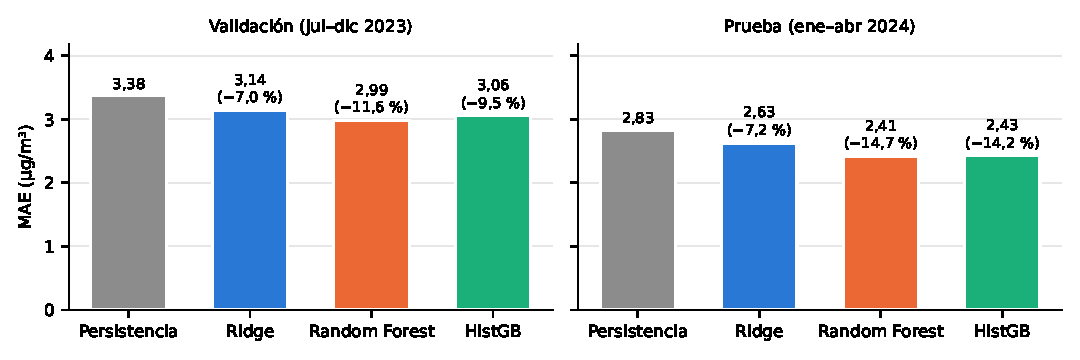
\includegraphics[width=\textwidth]{figures/15_comparacion_modelos.pdf}
\caption{MAE por modelo y bloque. Entre paréntesis, la reducción del MAE frente a la persistencia en el mismo bloque.}
\label{fig:comparacion}
\end{figure*}

El MAE de prueba es menor que el de validación para todos los modelos, incluida la persistencia, y el $R^2$ también es menor. Ambos hechos se explican por el cambio de distribución descrito en la sección~\ref{sec:eda}: enero--abril de 2024 tiene concentraciones más bajas y menos variables, de modo que los errores absolutos se reducen sin que el problema sea más fácil en términos relativos. Por la misma razón, el MAE de la validación cruzada interna (4,82 para Random Forest) es mayor: su primera ventana, en el invierno de 2022, tiene un MAE de 6,68, frente a 3,42 en la tercera.

\subsection{Aporte del calendario}
\label{sec:calendario}
La Tabla~\ref{tab:calendario} compara cada familia con y sin calendario en validación, con la misma búsqueda de hiperparámetros. En los modelos lineales el calendario empeora el MAE alrededor de un 2~\%, con un intervalo que excluye el cero; en los de árboles lo mejora un 3,2~\% (Random Forest) y un 2,4~\% (HistGB), también con intervalos que excluyen el cero. La importancia por permutación (Fig.~\ref{fig:importancia}) localiza el aporte en la hora pronosticada: permutarla aumenta el MAE de validación en 0,36 µg/m³ en Random Forest y 0,49 en HistGB, mientras que permutar el día de la semana no lo cambia. Una interpretación coherente es que el efecto de la hora no es aditivo: las mayores ganancias de los árboles sobre Ridge se concentran entre las 17 y las 21~h (sección~\ref{sec:errores}), cuando la concentración cambia de tendencia a diario, y esa interacción entre hora y nivel reciente no puede representarse con un seno y un coseno sumados linealmente.

\begin{table}[t]
\centering
\caption{MAE de validación sin y con calendario. $\Delta$: con menos sin (µg/m³), IC 95~\% por bootstrap de bloques.}
\label{tab:calendario}
\small
\setlength{\tabcolsep}{3pt}
\begin{tabular}{@{}lrrrl@{}}
\toprule
Familia & Sin & Con & Cambio & $\Delta$ [IC 95~\%] \\
\midrule
Ridge & 3,141 & 3,205 & $+2{,}0$~\% & $0{,}06$ [$0{,}02$; $0{,}11$] \\
Lasso & 3,142 & 3,205 & $+2{,}0$~\% & $0{,}06$ [$0{,}02$; $0{,}11$] \\
Random Forest & 3,083 & 2,985 & $-3{,}2$~\% & $-0{,}10$ [$-0{,}13$; $-0{,}06$] \\
HistGB & 3,132 & 3,057 & $-2{,}4$~\% & $-0{,}07$ [$-0{,}12$; $-0{,}02$] \\
\bottomrule
\end{tabular}
\end{table}

\subsection{Importancia de variables}
\label{sec:importancia}
La importancia se mide como el aumento del MAE de validación al permutar una variable, con 20 repeticiones (Fig.~\ref{fig:importancia}); para la hora y el día se permuta la variable original, de modo que su seno y coseno, o sus indicadores, se alteran juntos. En ambos modelos domina la medición actual: permutarla eleva el MAE en 6,76 (Random Forest) y 6,97 µg/m³ (HistGB). Le siguen la hora (0,36 y 0,49) y el rezago de una hora (0,28 y 0,33); el resto aporta menos de 0,15. Este patrón coincide con la autocorrelación parcial de la sección~\ref{sec:eda}, en la que la dependencia se concentra en los primeros rezagos.

\begin{figure}[t]
\centering
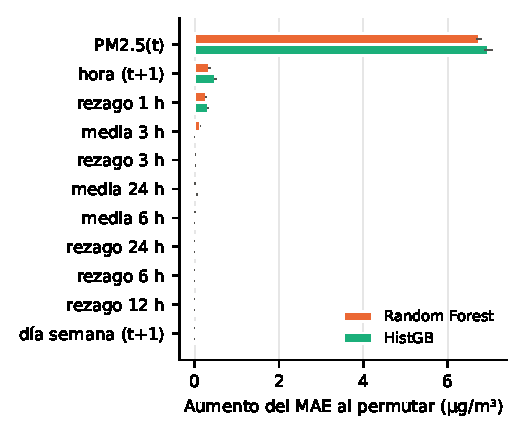
\includegraphics[width=\columnwidth]{figures/16_importancia_variables.pdf}
\caption{Importancia por permutación en validación: aumento del MAE al permutar cada variable (media y desviación de 20 repeticiones).}
\label{fig:importancia}
\end{figure}

Estas cifras tienen tres limitaciones. Primero, las variables de historial están muy correlacionadas: permutar una sola crea combinaciones de entrada que no ocurren en los datos y, a la vez, sus sustitutas pueden compensar su ausencia. Una importancia baja de, por ejemplo, la media de 6~h no implica que la variable sea irrelevante, sino que su información ya está en otras. La distorsión es visible en HistGB, donde permutar conjuntamente las nueve variables de historial aumenta el MAE menos (6,49) que permutar solo la medición actual (6,97). Segundo, la importancia por impureza de Random Forest, calculada en entrenamiento, ordena las variables de forma distinta (medición actual 0,65, media de 3~h 0,21 y rezago de 1~h 0,08) porque reparte el mérito entre variables correlacionadas y favorece las continuas; por eso se reporta solo como contraste. Tercero, ninguna de estas medidas es causal: describen de qué depende el modelo, no qué determina la concentración.

\subsection{Análisis de errores por hora y por mes}
\label{sec:errores}
La Fig.~\ref{fig:hora-mes} desagrega el MAE. Por hora, todos los modelos fallan más entre las 12 y las 15~h de validación, con MAE de 3,7 a 4,8 µg/m³, cuando la concentración sube y cambia con rapidez. La persistencia, que repite el último valor, sufre además en las transiciones: alcanza 5,07 a las 17~h y 3,35 a la 1~h. Allí los árboles obtienen sus mayores ganancias: a las 17~h Random Forest baja a 3,66 frente a 3,95 de Ridge, y a las 19~h, a 2,28 frente a 2,98. En la madrugada y la mañana (3 a 9~h) los cuatro modelos se comportan de forma muy parecida, y entre las 4 y las 7~h la persistencia es incluso ligeramente mejor, lo que indica que en ese tramo la serie cambia poco y la información adicional no aporta.

Por mes, el error es mayor entre septiembre y octubre de 2023 (MAE de 3,2 a 3,6 en todos los modelos) y mínimo en febrero de 2024 (1,9 a 2,1), y vuelve a subir en marzo y abril de 2024. Las diferencias entre meses son mayores que las diferencias entre modelos, por lo que el periodo evaluado condiciona la cifra global tanto como el modelo elegido. El orden de los modelos se mantiene casi todos los meses: la persistencia es la peor en los diez meses, y Random Forest supera a Ridge en nueve, con septiembre de 2023 como excepción.

\begin{figure*}[t]
\centering
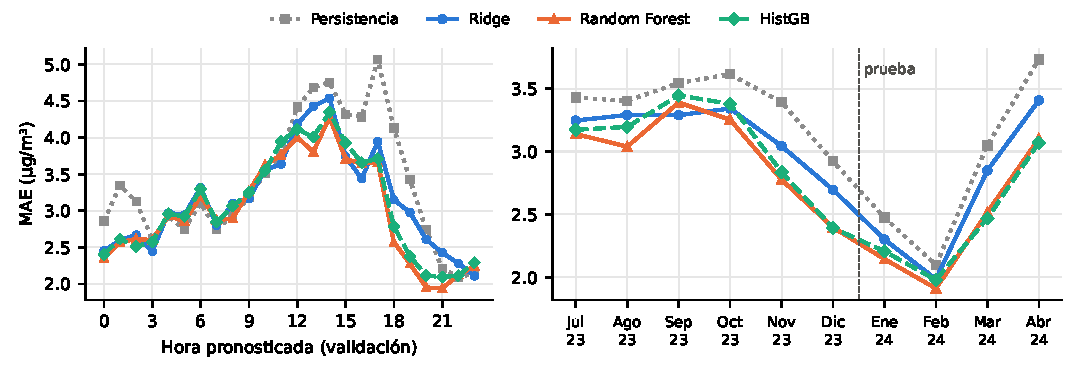
\includegraphics[width=\textwidth]{figures/17_errores_hora_mes.pdf}
\caption{MAE por hora pronosticada en validación (izquierda) y por mes en validación y prueba (derecha). La línea discontinua separa ambos bloques.}
\label{fig:hora-mes}
\end{figure*}

\subsection{Régimen de concentraciones altas}
\label{sec:regimen-alto}
La Fig.~\ref{fig:nivel} agrupa las horas según la concentración observada, usando como cortes la guía diaria de la OMS y sus metas intermedias~\cite{who_aqg_2021}; 50 µg/m³ coincide además con el ECA peruano~\cite{minam_eca_2017}. Esos valores se definen sobre promedios de 24~h y aquí solo sirven para agrupar horas. El MAE crece con la concentración en todos los modelos, y por encima de 50 µg/m³ el sesgo es claramente negativo: los modelos subestiman los episodios. Parte de ese sesgo es mecánica, porque agrupar por el valor observado selecciona las horas en que la concentración subió por encima de lo esperable con la información disponible, y cualquier predictor regresa hacia la media en ellas. Aun así, describe lo que ocurriría en un episodio real.

\begin{figure*}[t]
\centering
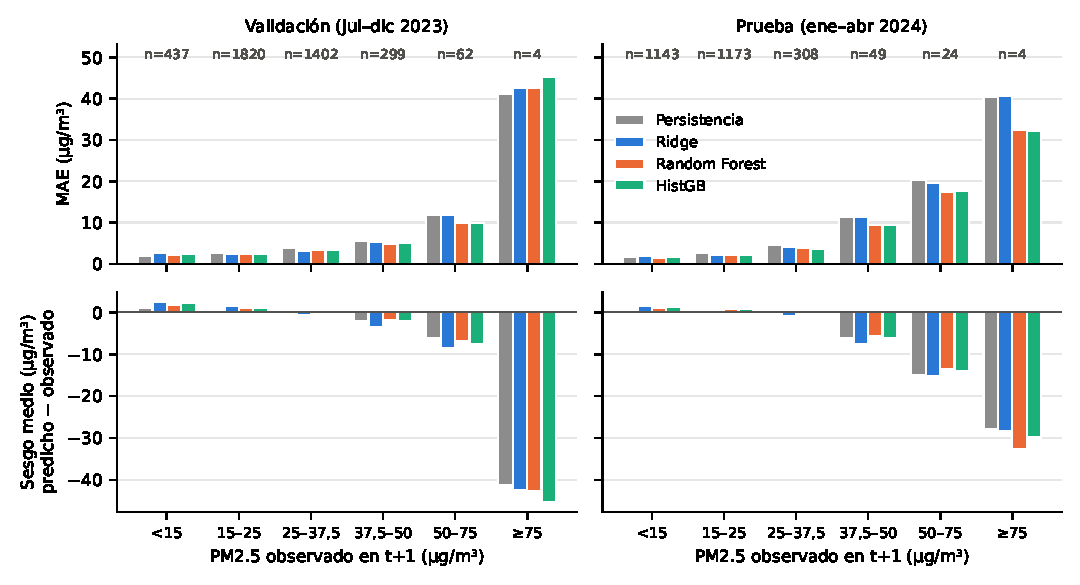
\includegraphics[width=\textwidth]{figures/18_errores_por_nivel.pdf}
\caption{MAE (arriba) y sesgo medio, predicho menos observado (abajo), por nivel de PM2.5 observado en $t+1$. Se indica el número de horas de cada nivel; el último tramo tiene solo cuatro horas por bloque.}
\label{fig:nivel}
\end{figure*}

La Tabla~\ref{tab:regimen} evalúa dos definiciones del régimen alto. La primera es un umbral fijo de 59,25 µg/m³, el percentil 90 de la respuesta en entrenamiento; por el descenso de las concentraciones solo lo superan 16 horas de validación y 17 de prueba. La segunda es el decil superior de cada bloque (desde 36,8 µg/m³ en validación y 27,5 en prueba), con muestra suficiente para comparar. En el decil superior el MAE es entre dos y cuatro veces el del resto de horas (por ejemplo, 5,89 frente a 2,66 para Random Forest en validación y 6,80 frente a 1,92 en prueba). Random Forest y HistGB mejoran a la persistencia en ese decil entre un 8,7~\% y un 18,3~\%, con intervalos que excluyen el cero en ambos bloques, mientras que la mejora de Ridge es pequeña (1,7~\% y 5,3~\%) y en validación no se distingue de cero. Con el umbral fijo, en prueba los árboles reducen el MAE en unos 5,5 µg/m³ frente a la persistencia (IC $[-7{,}8;\,-2{,}5]$ para Random Forest), pero su sesgo sigue cerca de $-22{,}5$ µg/m³; en validación ninguna diferencia es concluyente. Con tan pocas horas, estas cifras son indicativas.

\begin{table}[t]
\centering
\caption{Régimen alto. Umbral fijo: respuesta $\geq 59{,}25$ µg/m³ (p90 de entrenamiento). Decil: 10~\% superior de cada bloque. Mejora frente a persistencia; * indica que el IC 95~\% de la diferencia de MAE excluye el cero.}
\label{tab:regimen}
\small
\setlength{\tabcolsep}{3pt}
\begin{tabular}{@{}lrrrrrr@{}}
\toprule
& \multicolumn{2}{c}{Decil, val.} & \multicolumn{2}{c}{Decil, prueba} & \multicolumn{2}{c}{Umbral, prueba} \\
\cmidrule(lr){2-3}\cmidrule(lr){4-5}\cmidrule(l){6-7}
Modelo & MAE & Mejora & MAE & Mejora & MAE & Mejora \\
\midrule
$n$ & \multicolumn{2}{c}{403} & \multicolumn{2}{c}{272} & \multicolumn{2}{c}{17} \\
Persistencia & 6,74 & -- & 8,08 & -- & 29,05 & -- \\
Ridge & 6,63 & 1,7~\% & 7,65 & 5,3~\%* & 28,28 & 2,6~\% \\
Random Forest & 5,89 & 12,6~\%* & 6,80 & 15,9~\%* & 23,50 & 19,1~\%* \\
HistGB & 6,15 & 8,7~\%* & 6,59 & 18,3~\%* & 23,44 & 19,3~\%* \\
\bottomrule
\end{tabular}
\end{table}

La subestimación persistente es coherente con la limitación señalada en la sección~\ref{sec:no-lineales}: los árboles promedian valores observados en hojas grandes y no pueden anticipar un pico que la historia reciente no anuncia. Sin variables meteorológicas ni de emisiones, el historial de la propia serie no contiene la información necesaria para prever el inicio de un episodio.

\subsection{Respuesta a las preguntas de investigación}
\label{sec:respuestas}
\textbf{PI1.} Los modelos de árboles mejoran a la persistencia entre un 9,5~\% y un 11,6~\% en MAE en validación y alrededor de un 14~\% en prueba (unos 0,4 µg/m³ por hora), frente al 7~\% de Ridge. La mejora es estadísticamente consistente, pero pequeña en términos absolutos: la persistencia sigue siendo una referencia exigente a una hora.

\textbf{PI2.} El calendario aporta solo en los modelos que pueden combinarlo con el historial. En los de árboles reduce el MAE de validación un 2--3~\%, y el aporte proviene de la hora pronosticada; el día de la semana no aporta en ningún modelo. En los lineales, el calendario empeora ligeramente el MAE.

\textbf{PI3.} Sí. En el decil superior el MAE es entre dos y cuatro veces el del resto, y por encima de 50 µg/m³ todos los modelos subestiman de forma sistemática. Los árboles conservan, e incluso amplían, su ventaja relativa sobre la persistencia en ese régimen; la de Ridge se reduce a un 2--5~\% y en validación no se distingue de cero. Ningún modelo resuelve la subestimación de los picos, que es la principal limitación para un uso sanitario del pronóstico.
.
% Requiere booktabs y graphicx. Figuras 15-18: scripts/06_analisis_errores.py.
% Cifras: data/processed/lineales_*.csv, no_lineales_*.csv y errores_*.csv.
\section{Resultados y análisis}
\label{sec:resultados}
Se comparan cuatro modelos sobre las mismas filas: persistencia, Ridge sin calendario (el lineal elegido en la sección~\ref{sec:metodologia}) y los representantes con calendario de Random Forest y HistGB. Las diferencias de MAE se acompañan de intervalos de confianza del 95~\% obtenidos por bootstrap de bloques móviles de 24 filas consecutivas (2000 réplicas), que conserva la autocorrelación de los errores; los bloques se forman sobre filas, por lo que un hueco de medición puede quedar dentro de un bloque.

\subsection{Comparación global}
\label{sec:comparacion}
La Tabla~\ref{tab:resultados} y la Fig.~\ref{fig:comparacion} resumen el desempeño. En validación, Random Forest obtiene el menor MAE (2,985) y mejora un 11,6~\% sobre la persistencia, frente al 9,5~\% de HistGB y el 7,0~\% de Ridge. En prueba, los dos modelos de árboles quedan prácticamente empatados en MAE (2,413 y 2,428, mejoras de 14,7~\% y 14,2~\%) y HistGB logra el menor RMSE (4,347). Los intervalos de la diferencia con la persistencia excluyen el cero para los tres modelos en ambos bloques. Frente a Ridge, Random Forest reduce el MAE en 0,16 µg/m³ en validación (IC $[-0{,}22;\,-0{,}10]$) y 0,21 en prueba ($[-0{,}28;\,-0{,}15]$); HistGB, en 0,08 ($[-0{,}15;\,-0{,}02]$) y 0,20 ($[-0{,}27;\,-0{,}12]$). La ganancia de los árboles es, por tanto, consistente pero modesta en términos absolutos: del orden de 0,2--0,4 µg/m³ por hora.

\begin{table}[t]
\centering
\caption{Desempeño en validación y prueba. Mejora: reducción porcentual del MAE frente a la persistencia en el mismo bloque. $\Delta$: diferencia de MAE frente a persistencia (µg/m³) con IC 95~\% por bootstrap de bloques.}
\label{tab:resultados}
\small
\setlength{\tabcolsep}{3.5pt}
\begin{tabular}{@{}lrrrrl@{}}
\toprule
Modelo & MAE & RMSE & $R^2$ & Mejora & $\Delta$ [IC 95~\%] \\
\midrule
\multicolumn{6}{@{}l}{\emph{Validación (jul--dic 2023, $n=4024$)}} \\
Persistencia & 3,378 & 5,143 & 0,700 & -- & -- \\
Ridge & 3,141 & 4,755 & 0,744 & 7,0~\% & $-0{,}24$ [$-0{,}29$; $-0{,}18$] \\
Random Forest & \textbf{2,985} & \textbf{4,565} & \textbf{0,764} & 11,6~\% & $-0{,}39$ [$-0{,}47$; $-0{,}32$] \\
HistGB & 3,057 & 4,617 & 0,758 & 9,5~\% & $-0{,}32$ [$-0{,}41$; $-0{,}24$] \\
\midrule
\multicolumn{6}{@{}l}{\emph{Prueba (ene--abr 2024, $n=2701$)}} \\
Persistencia & 2,829 & 5,265 & 0,631 & -- & -- \\
Ridge & 2,626 & 4,766 & 0,698 & 7,2~\% & $-0{,}20$ [$-0{,}27$; $-0{,}13$] \\
Random Forest & \textbf{2,413} & 4,486 & 0,732 & 14,7~\% & $-0{,}42$ [$-0{,}51$; $-0{,}31$] \\
HistGB & 2,428 & \textbf{4,347} & \textbf{0,749} & 14,2~\% & $-0{,}40$ [$-0{,}52$; $-0{,}28$] \\
\bottomrule
\end{tabular}
\end{table}

\begin{figure*}[t]
\centering
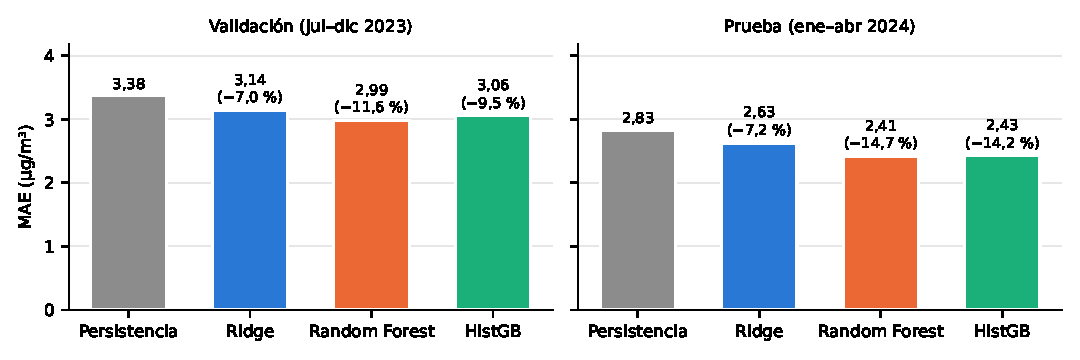
\includegraphics[width=\textwidth]{figures/15_comparacion_modelos.pdf}
\caption{MAE por modelo y bloque. Entre paréntesis, la reducción del MAE frente a la persistencia en el mismo bloque.}
\label{fig:comparacion}
\end{figure*}

El MAE de prueba es menor que el de validación para todos los modelos, incluida la persistencia, y el $R^2$ también es menor. Ambos hechos se explican por el cambio de distribución descrito en la sección~\ref{sec:eda}: enero--abril de 2024 tiene concentraciones más bajas y menos variables, de modo que los errores absolutos se reducen sin que el problema sea más fácil en términos relativos. Por la misma razón, el MAE de la validación cruzada interna (4,82 para Random Forest) es mayor: su primera ventana, en el invierno de 2022, tiene un MAE de 6,68, frente a 3,42 en la tercera.

\subsection{Aporte del calendario}
\label{sec:calendario}
La Tabla~\ref{tab:calendario} compara cada familia con y sin calendario en validación, con la misma búsqueda de hiperparámetros. En los modelos lineales el calendario empeora el MAE alrededor de un 2~\%, con un intervalo que excluye el cero; en los de árboles lo mejora un 3,2~\% (Random Forest) y un 2,4~\% (HistGB), también con intervalos que excluyen el cero. La importancia por permutación (Fig.~\ref{fig:importancia}) localiza el aporte en la hora pronosticada: permutarla aumenta el MAE de validación en 0,36 µg/m³ en Random Forest y 0,49 en HistGB, mientras que permutar el día de la semana no lo cambia. Una interpretación coherente es que el efecto de la hora no es aditivo: las mayores ganancias de los árboles sobre Ridge se concentran entre las 17 y las 21~h (sección~\ref{sec:errores}), cuando la concentración cambia de tendencia a diario, y esa interacción entre hora y nivel reciente no puede representarse con un seno y un coseno sumados linealmente.

\begin{table}[t]
\centering
\caption{MAE de validación sin y con calendario. $\Delta$: con menos sin (µg/m³), IC 95~\% por bootstrap de bloques.}
\label{tab:calendario}
\small
\setlength{\tabcolsep}{3pt}
\begin{tabular}{@{}lrrrl@{}}
\toprule
Familia & Sin & Con & Cambio & $\Delta$ [IC 95~\%] \\
\midrule
Ridge & 3,141 & 3,205 & $+2{,}0$~\% & $0{,}06$ [$0{,}02$; $0{,}11$] \\
Lasso & 3,142 & 3,205 & $+2{,}0$~\% & $0{,}06$ [$0{,}02$; $0{,}11$] \\
Random Forest & 3,083 & 2,985 & $-3{,}2$~\% & $-0{,}10$ [$-0{,}13$; $-0{,}06$] \\
HistGB & 3,132 & 3,057 & $-2{,}4$~\% & $-0{,}07$ [$-0{,}12$; $-0{,}02$] \\
\bottomrule
\end{tabular}
\end{table}

\subsection{Importancia de variables}
\label{sec:importancia}
La importancia se mide como el aumento del MAE de validación al permutar una variable, con 20 repeticiones (Fig.~\ref{fig:importancia}); para la hora y el día se permuta la variable original, de modo que su seno y coseno, o sus indicadores, se alteran juntos. En ambos modelos domina la medición actual: permutarla eleva el MAE en 6,76 (Random Forest) y 6,97 µg/m³ (HistGB). Le siguen la hora (0,36 y 0,49) y el rezago de una hora (0,28 y 0,33); el resto aporta menos de 0,15. Este patrón coincide con la autocorrelación parcial de la sección~\ref{sec:eda}, en la que la dependencia se concentra en los primeros rezagos.

\begin{figure}[t]
\centering
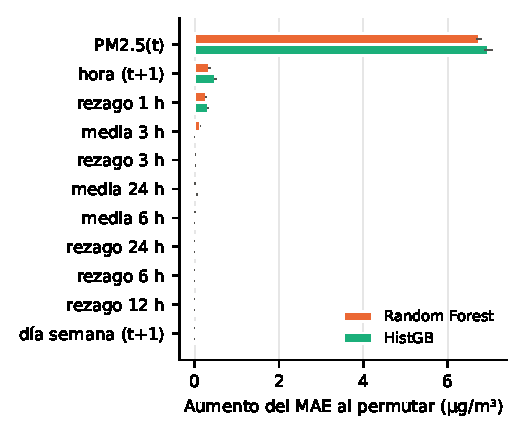
\includegraphics[width=\columnwidth]{figures/16_importancia_variables.pdf}
\caption{Importancia por permutación en validación: aumento del MAE al permutar cada variable (media y desviación de 20 repeticiones).}
\label{fig:importancia}
\end{figure}

Estas cifras tienen tres limitaciones. Primero, las variables de historial están muy correlacionadas: permutar una sola crea combinaciones de entrada que no ocurren en los datos y, a la vez, sus sustitutas pueden compensar su ausencia. Una importancia baja de, por ejemplo, la media de 6~h no implica que la variable sea irrelevante, sino que su información ya está en otras. La distorsión es visible en HistGB, donde permutar conjuntamente las nueve variables de historial aumenta el MAE menos (6,49) que permutar solo la medición actual (6,97). Segundo, la importancia por impureza de Random Forest, calculada en entrenamiento, ordena las variables de forma distinta (medición actual 0,65, media de 3~h 0,21 y rezago de 1~h 0,08) porque reparte el mérito entre variables correlacionadas y favorece las continuas; por eso se reporta solo como contraste. Tercero, ninguna de estas medidas es causal: describen de qué depende el modelo, no qué determina la concentración.

\subsection{Análisis de errores por hora y por mes}
\label{sec:errores}
La Fig.~\ref{fig:hora-mes} desagrega el MAE. Por hora, todos los modelos fallan más entre las 12 y las 15~h de validación, con MAE de 3,7 a 4,8 µg/m³, cuando la concentración sube y cambia con rapidez. La persistencia, que repite el último valor, sufre además en las transiciones: alcanza 5,07 a las 17~h y 3,35 a la 1~h. Allí los árboles obtienen sus mayores ganancias: a las 17~h Random Forest baja a 3,66 frente a 3,95 de Ridge, y a las 19~h, a 2,28 frente a 2,98. En la madrugada y la mañana (3 a 9~h) los cuatro modelos se comportan de forma muy parecida, y entre las 4 y las 7~h la persistencia es incluso ligeramente mejor, lo que indica que en ese tramo la serie cambia poco y la información adicional no aporta.

Por mes, el error es mayor entre septiembre y octubre de 2023 (MAE de 3,2 a 3,6 en todos los modelos) y mínimo en febrero de 2024 (1,9 a 2,1), y vuelve a subir en marzo y abril de 2024. Las diferencias entre meses son mayores que las diferencias entre modelos, por lo que el periodo evaluado condiciona la cifra global tanto como el modelo elegido. El orden de los modelos se mantiene casi todos los meses: la persistencia es la peor en los diez meses, y Random Forest supera a Ridge en nueve, con septiembre de 2023 como excepción.

\begin{figure*}[t]
\centering
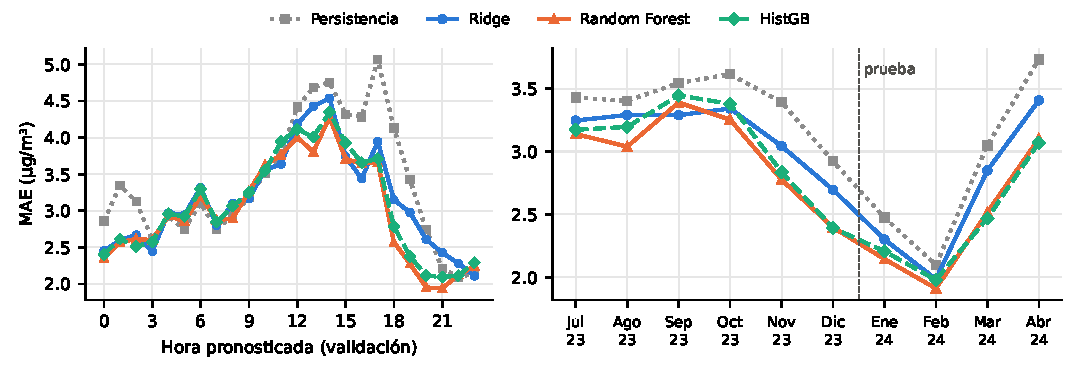
\includegraphics[width=\textwidth]{figures/17_errores_hora_mes.pdf}
\caption{MAE por hora pronosticada en validación (izquierda) y por mes en validación y prueba (derecha). La línea discontinua separa ambos bloques.}
\label{fig:hora-mes}
\end{figure*}

\subsection{Régimen de concentraciones altas}
\label{sec:regimen-alto}
La Fig.~\ref{fig:nivel} agrupa las horas según la concentración observada, usando como cortes la guía diaria de la OMS y sus metas intermedias~\cite{who_aqg_2021}; 50 µg/m³ coincide además con el ECA peruano~\cite{minam_eca_2017}. Esos valores se definen sobre promedios de 24~h y aquí solo sirven para agrupar horas. El MAE crece con la concentración en todos los modelos, y por encima de 50 µg/m³ el sesgo es claramente negativo: los modelos subestiman los episodios. Parte de ese sesgo es mecánica, porque agrupar por el valor observado selecciona las horas en que la concentración subió por encima de lo esperable con la información disponible, y cualquier predictor regresa hacia la media en ellas. Aun así, describe lo que ocurriría en un episodio real.

\begin{figure*}[t]
\centering
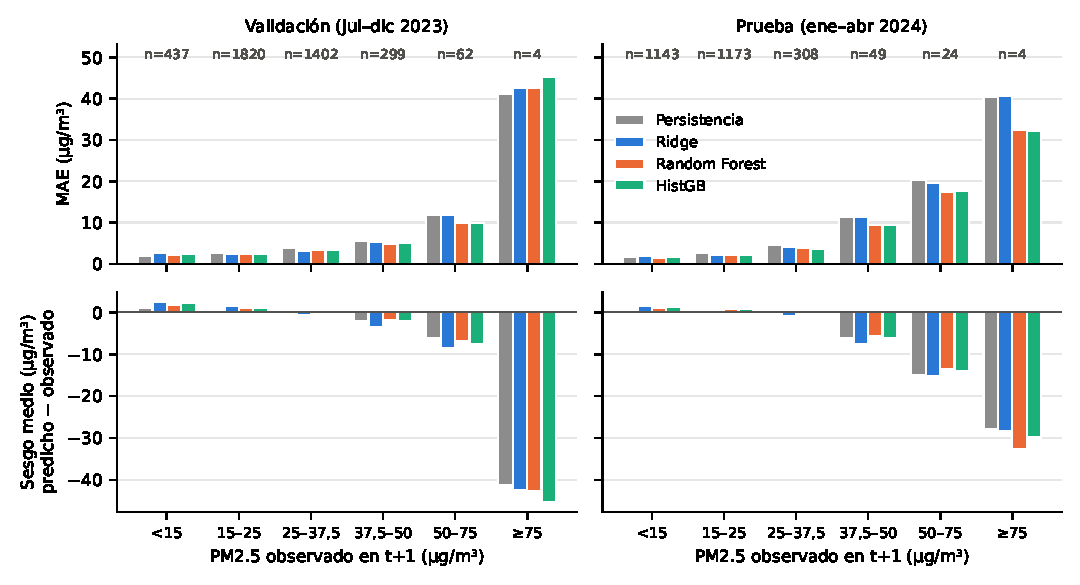
\includegraphics[width=\textwidth]{figures/18_errores_por_nivel.pdf}
\caption{MAE (arriba) y sesgo medio, predicho menos observado (abajo), por nivel de PM2.5 observado en $t+1$. Se indica el número de horas de cada nivel; el último tramo tiene solo cuatro horas por bloque.}
\label{fig:nivel}
\end{figure*}

La Tabla~\ref{tab:regimen} evalúa dos definiciones del régimen alto. La primera es un umbral fijo de 59,25 µg/m³, el percentil 90 de la respuesta en entrenamiento; por el descenso de las concentraciones solo lo superan 16 horas de validación y 17 de prueba. La segunda es el decil superior de cada bloque (desde 36,8 µg/m³ en validación y 27,5 en prueba), con muestra suficiente para comparar. En el decil superior el MAE es entre dos y cuatro veces el del resto de horas (por ejemplo, 5,89 frente a 2,66 para Random Forest en validación y 6,80 frente a 1,92 en prueba). Random Forest y HistGB mejoran a la persistencia en ese decil entre un 8,7~\% y un 18,3~\%, con intervalos que excluyen el cero en ambos bloques, mientras que la mejora de Ridge es pequeña (1,7~\% y 5,3~\%) y en validación no se distingue de cero. Con el umbral fijo, en prueba los árboles reducen el MAE en unos 5,5 µg/m³ frente a la persistencia (IC $[-7{,}8;\,-2{,}5]$ para Random Forest), pero su sesgo sigue cerca de $-22{,}5$ µg/m³; en validación ninguna diferencia es concluyente. Con tan pocas horas, estas cifras son indicativas.

\begin{table}[t]
\centering
\caption{Régimen alto. Umbral fijo: respuesta $\geq 59{,}25$ µg/m³ (p90 de entrenamiento). Decil: 10~\% superior de cada bloque. Mejora frente a persistencia; * indica que el IC 95~\% de la diferencia de MAE excluye el cero.}
\label{tab:regimen}
\small
\setlength{\tabcolsep}{3pt}
\begin{tabular}{@{}lrrrrrr@{}}
\toprule
& \multicolumn{2}{c}{Decil, val.} & \multicolumn{2}{c}{Decil, prueba} & \multicolumn{2}{c}{Umbral, prueba} \\
\cmidrule(lr){2-3}\cmidrule(lr){4-5}\cmidrule(l){6-7}
Modelo & MAE & Mejora & MAE & Mejora & MAE & Mejora \\
\midrule
$n$ & \multicolumn{2}{c}{403} & \multicolumn{2}{c}{272} & \multicolumn{2}{c}{17} \\
Persistencia & 6,74 & -- & 8,08 & -- & 29,05 & -- \\
Ridge & 6,63 & 1,7~\% & 7,65 & 5,3~\%* & 28,28 & 2,6~\% \\
Random Forest & 5,89 & 12,6~\%* & 6,80 & 15,9~\%* & 23,50 & 19,1~\%* \\
HistGB & 6,15 & 8,7~\%* & 6,59 & 18,3~\%* & 23,44 & 19,3~\%* \\
\bottomrule
\end{tabular}
\end{table}

La subestimación persistente es coherente con la limitación señalada en la sección~\ref{sec:no-lineales}: los árboles promedian valores observados en hojas grandes y no pueden anticipar un pico que la historia reciente no anuncia. Sin variables meteorológicas ni de emisiones, el historial de la propia serie no contiene la información necesaria para prever el inicio de un episodio.

\subsection{Respuesta a las preguntas de investigación}
\label{sec:respuestas}
\textbf{PI1.} Los modelos de árboles mejoran a la persistencia entre un 9,5~\% y un 11,6~\% en MAE en validación y alrededor de un 14~\% en prueba (unos 0,4 µg/m³ por hora), frente al 7~\% de Ridge. La mejora es estadísticamente consistente, pero pequeña en términos absolutos: la persistencia sigue siendo una referencia exigente a una hora.

\textbf{PI2.} El calendario aporta solo en los modelos que pueden combinarlo con el historial. En los de árboles reduce el MAE de validación un 2--3~\%, y el aporte proviene de la hora pronosticada; el día de la semana no aporta en ningún modelo. En los lineales, el calendario empeora ligeramente el MAE.

\textbf{PI3.} Sí. En el decil superior el MAE es entre dos y cuatro veces el del resto, y por encima de 50 µg/m³ todos los modelos subestiman de forma sistemática. Los árboles conservan, e incluso amplían, su ventaja relativa sobre la persistencia en ese régimen; la de Ridge se reduce a un 2--5~\% y en validación no se distingue de cero. Ningún modelo resuelve la subestimación de los picos, que es la principal limitación para un uso sanitario del pronóstico.
.
% Requiere booktabs y graphicx. Figuras 15-18: scripts/06_analisis_errores.py.
% Cifras: data/processed/lineales_*.csv, no_lineales_*.csv y errores_*.csv.
\section{Resultados y análisis}
\label{sec:resultados}
Se comparan cuatro modelos sobre las mismas filas: persistencia, Ridge sin calendario (el lineal elegido en la sección~\ref{sec:metodologia}) y los representantes con calendario de Random Forest y HistGB. Las diferencias de MAE se acompañan de intervalos de confianza del 95~\% obtenidos por bootstrap de bloques móviles de 24 filas consecutivas (2000 réplicas), que conserva la autocorrelación de los errores; los bloques se forman sobre filas, por lo que un hueco de medición puede quedar dentro de un bloque.

\subsection{Comparación global}
\label{sec:comparacion}
La Tabla~\ref{tab:resultados} y la Fig.~\ref{fig:comparacion} resumen el desempeño. En validación, Random Forest obtiene el menor MAE (2,985) y mejora un 11,6~\% sobre la persistencia, frente al 9,5~\% de HistGB y el 7,0~\% de Ridge. En prueba, los dos modelos de árboles quedan prácticamente empatados en MAE (2,413 y 2,428, mejoras de 14,7~\% y 14,2~\%) y HistGB logra el menor RMSE (4,347). Los intervalos de la diferencia con la persistencia excluyen el cero para los tres modelos en ambos bloques. Frente a Ridge, Random Forest reduce el MAE en 0,16 µg/m³ en validación (IC $[-0{,}22;\,-0{,}10]$) y 0,21 en prueba ($[-0{,}28;\,-0{,}15]$); HistGB, en 0,08 ($[-0{,}15;\,-0{,}02]$) y 0,20 ($[-0{,}27;\,-0{,}12]$). La ganancia de los árboles es, por tanto, consistente pero modesta en términos absolutos: del orden de 0,2--0,4 µg/m³ por hora.

\begin{table}[t]
\centering
\caption{Desempeño en validación y prueba. Mejora: reducción porcentual del MAE frente a la persistencia en el mismo bloque. $\Delta$: diferencia de MAE frente a persistencia (µg/m³) con IC 95~\% por bootstrap de bloques.}
\label{tab:resultados}
\small
\setlength{\tabcolsep}{3.5pt}
\begin{tabular}{@{}lrrrrl@{}}
\toprule
Modelo & MAE & RMSE & $R^2$ & Mejora & $\Delta$ [IC 95~\%] \\
\midrule
\multicolumn{6}{@{}l}{\emph{Validación (jul--dic 2023, $n=4024$)}} \\
Persistencia & 3,378 & 5,143 & 0,700 & -- & -- \\
Ridge & 3,141 & 4,755 & 0,744 & 7,0~\% & $-0{,}24$ [$-0{,}29$; $-0{,}18$] \\
Random Forest & \textbf{2,985} & \textbf{4,565} & \textbf{0,764} & 11,6~\% & $-0{,}39$ [$-0{,}47$; $-0{,}32$] \\
HistGB & 3,057 & 4,617 & 0,758 & 9,5~\% & $-0{,}32$ [$-0{,}41$; $-0{,}24$] \\
\midrule
\multicolumn{6}{@{}l}{\emph{Prueba (ene--abr 2024, $n=2701$)}} \\
Persistencia & 2,829 & 5,265 & 0,631 & -- & -- \\
Ridge & 2,626 & 4,766 & 0,698 & 7,2~\% & $-0{,}20$ [$-0{,}27$; $-0{,}13$] \\
Random Forest & \textbf{2,413} & 4,486 & 0,732 & 14,7~\% & $-0{,}42$ [$-0{,}51$; $-0{,}31$] \\
HistGB & 2,428 & \textbf{4,347} & \textbf{0,749} & 14,2~\% & $-0{,}40$ [$-0{,}52$; $-0{,}28$] \\
\bottomrule
\end{tabular}
\end{table}

\begin{figure*}[t]
\centering
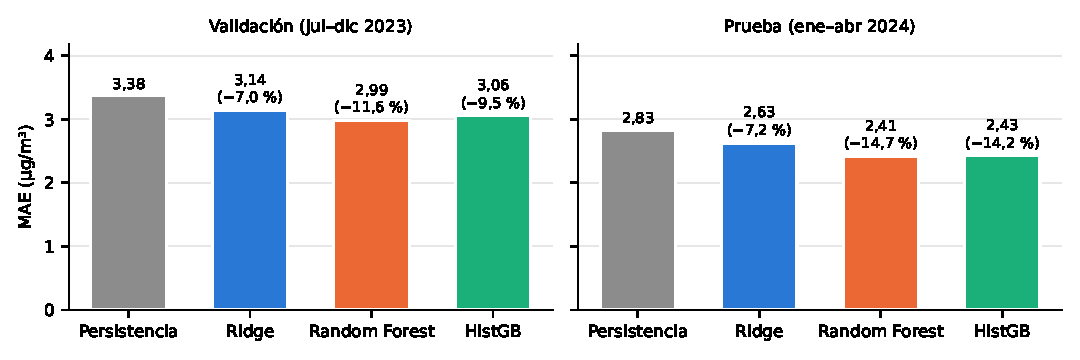
\includegraphics[width=\textwidth]{figures/15_comparacion_modelos.pdf}
\caption{MAE por modelo y bloque. Entre paréntesis, la reducción del MAE frente a la persistencia en el mismo bloque.}
\label{fig:comparacion}
\end{figure*}

El MAE de prueba es menor que el de validación para todos los modelos, incluida la persistencia, y el $R^2$ también es menor. Ambos hechos se explican por el cambio de distribución descrito en la sección~\ref{sec:eda}: enero--abril de 2024 tiene concentraciones más bajas y menos variables, de modo que los errores absolutos se reducen sin que el problema sea más fácil en términos relativos. Por la misma razón, el MAE de la validación cruzada interna (4,82 para Random Forest) es mayor: su primera ventana, en el invierno de 2022, tiene un MAE de 6,68, frente a 3,42 en la tercera.

\subsection{Aporte del calendario}
\label{sec:calendario}
La Tabla~\ref{tab:calendario} compara cada familia con y sin calendario en validación, con la misma búsqueda de hiperparámetros. En los modelos lineales el calendario empeora el MAE alrededor de un 2~\%, con un intervalo que excluye el cero; en los de árboles lo mejora un 3,2~\% (Random Forest) y un 2,4~\% (HistGB), también con intervalos que excluyen el cero. La importancia por permutación (Fig.~\ref{fig:importancia}) localiza el aporte en la hora pronosticada: permutarla aumenta el MAE de validación en 0,36 µg/m³ en Random Forest y 0,49 en HistGB, mientras que permutar el día de la semana no lo cambia. Una interpretación coherente es que el efecto de la hora no es aditivo: las mayores ganancias de los árboles sobre Ridge se concentran entre las 17 y las 21~h (sección~\ref{sec:errores}), cuando la concentración cambia de tendencia a diario, y esa interacción entre hora y nivel reciente no puede representarse con un seno y un coseno sumados linealmente.

\begin{table}[t]
\centering
\caption{MAE de validación sin y con calendario. $\Delta$: con menos sin (µg/m³), IC 95~\% por bootstrap de bloques.}
\label{tab:calendario}
\small
\setlength{\tabcolsep}{3pt}
\begin{tabular}{@{}lrrrl@{}}
\toprule
Familia & Sin & Con & Cambio & $\Delta$ [IC 95~\%] \\
\midrule
Ridge & 3,141 & 3,205 & $+2{,}0$~\% & $0{,}06$ [$0{,}02$; $0{,}11$] \\
Lasso & 3,142 & 3,205 & $+2{,}0$~\% & $0{,}06$ [$0{,}02$; $0{,}11$] \\
Random Forest & 3,083 & 2,985 & $-3{,}2$~\% & $-0{,}10$ [$-0{,}13$; $-0{,}06$] \\
HistGB & 3,132 & 3,057 & $-2{,}4$~\% & $-0{,}07$ [$-0{,}12$; $-0{,}02$] \\
\bottomrule
\end{tabular}
\end{table}

\subsection{Importancia de variables}
\label{sec:importancia}
La importancia se mide como el aumento del MAE de validación al permutar una variable, con 20 repeticiones (Fig.~\ref{fig:importancia}); para la hora y el día se permuta la variable original, de modo que su seno y coseno, o sus indicadores, se alteran juntos. En ambos modelos domina la medición actual: permutarla eleva el MAE en 6,76 (Random Forest) y 6,97 µg/m³ (HistGB). Le siguen la hora (0,36 y 0,49) y el rezago de una hora (0,28 y 0,33); el resto aporta menos de 0,15. Este patrón coincide con la autocorrelación parcial de la sección~\ref{sec:eda}, en la que la dependencia se concentra en los primeros rezagos.

\begin{figure}[t]
\centering
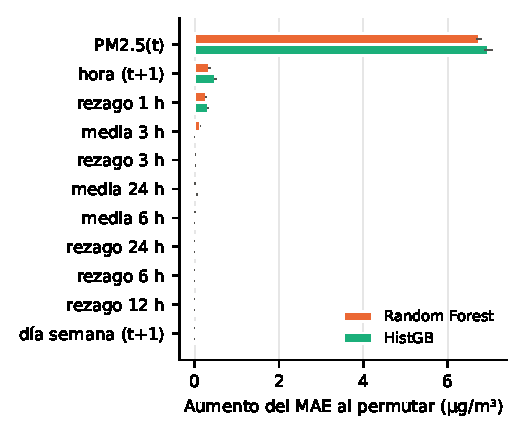
\includegraphics[width=\columnwidth]{figures/16_importancia_variables.pdf}
\caption{Importancia por permutación en validación: aumento del MAE al permutar cada variable (media y desviación de 20 repeticiones).}
\label{fig:importancia}
\end{figure}

Estas cifras tienen tres limitaciones. Primero, las variables de historial están muy correlacionadas: permutar una sola crea combinaciones de entrada que no ocurren en los datos y, a la vez, sus sustitutas pueden compensar su ausencia. Una importancia baja de, por ejemplo, la media de 6~h no implica que la variable sea irrelevante, sino que su información ya está en otras. La distorsión es visible en HistGB, donde permutar conjuntamente las nueve variables de historial aumenta el MAE menos (6,49) que permutar solo la medición actual (6,97). Segundo, la importancia por impureza de Random Forest, calculada en entrenamiento, ordena las variables de forma distinta (medición actual 0,65, media de 3~h 0,21 y rezago de 1~h 0,08) porque reparte el mérito entre variables correlacionadas y favorece las continuas; por eso se reporta solo como contraste. Tercero, ninguna de estas medidas es causal: describen de qué depende el modelo, no qué determina la concentración.

\subsection{Análisis de errores por hora y por mes}
\label{sec:errores}
La Fig.~\ref{fig:hora-mes} desagrega el MAE. Por hora, todos los modelos fallan más entre las 12 y las 15~h de validación, con MAE de 3,7 a 4,8 µg/m³, cuando la concentración sube y cambia con rapidez. La persistencia, que repite el último valor, sufre además en las transiciones: alcanza 5,07 a las 17~h y 3,35 a la 1~h. Allí los árboles obtienen sus mayores ganancias: a las 17~h Random Forest baja a 3,66 frente a 3,95 de Ridge, y a las 19~h, a 2,28 frente a 2,98. En la madrugada y la mañana (3 a 9~h) los cuatro modelos se comportan de forma muy parecida, y entre las 4 y las 7~h la persistencia es incluso ligeramente mejor, lo que indica que en ese tramo la serie cambia poco y la información adicional no aporta.

Por mes, el error es mayor entre septiembre y octubre de 2023 (MAE de 3,2 a 3,6 en todos los modelos) y mínimo en febrero de 2024 (1,9 a 2,1), y vuelve a subir en marzo y abril de 2024. Las diferencias entre meses son mayores que las diferencias entre modelos, por lo que el periodo evaluado condiciona la cifra global tanto como el modelo elegido. El orden de los modelos se mantiene casi todos los meses: la persistencia es la peor en los diez meses, y Random Forest supera a Ridge en nueve, con septiembre de 2023 como excepción.

\begin{figure*}[t]
\centering
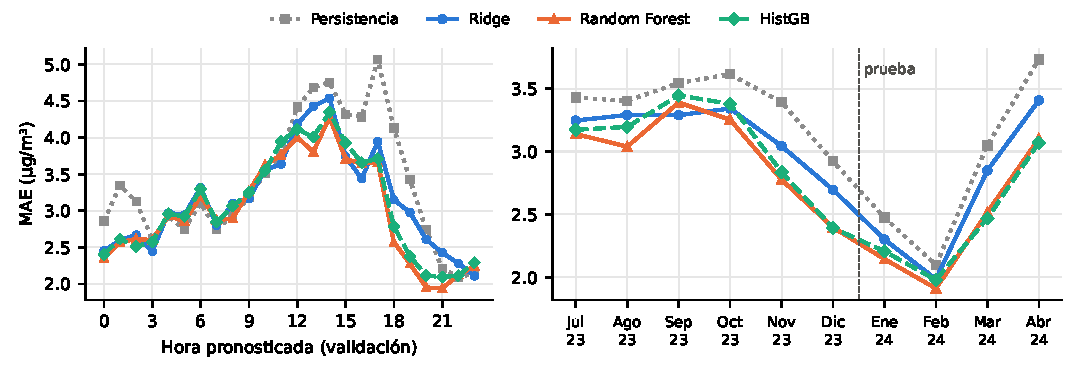
\includegraphics[width=\textwidth]{figures/17_errores_hora_mes.pdf}
\caption{MAE por hora pronosticada en validación (izquierda) y por mes en validación y prueba (derecha). La línea discontinua separa ambos bloques.}
\label{fig:hora-mes}
\end{figure*}

\subsection{Régimen de concentraciones altas}
\label{sec:regimen-alto}
La Fig.~\ref{fig:nivel} agrupa las horas según la concentración observada, usando como cortes la guía diaria de la OMS y sus metas intermedias~\cite{who_aqg_2021}; 50 µg/m³ coincide además con el ECA peruano~\cite{minam_eca_2017}. Esos valores se definen sobre promedios de 24~h y aquí solo sirven para agrupar horas. El MAE crece con la concentración en todos los modelos, y por encima de 50 µg/m³ el sesgo es claramente negativo: los modelos subestiman los episodios. Parte de ese sesgo es mecánica, porque agrupar por el valor observado selecciona las horas en que la concentración subió por encima de lo esperable con la información disponible, y cualquier predictor regresa hacia la media en ellas. Aun así, describe lo que ocurriría en un episodio real.

\begin{figure*}[t]
\centering
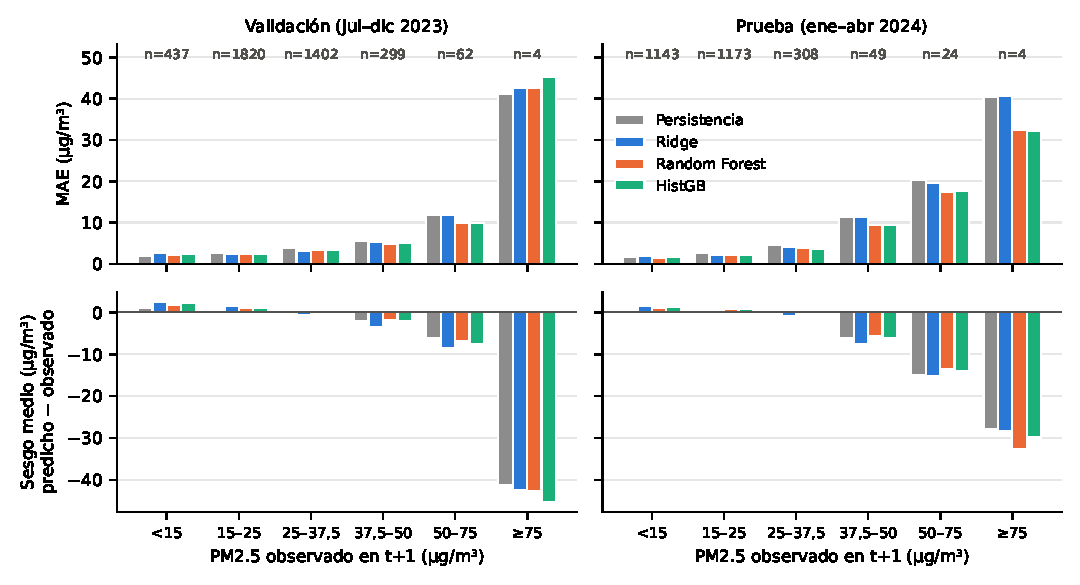
\includegraphics[width=\textwidth]{figures/18_errores_por_nivel.pdf}
\caption{MAE (arriba) y sesgo medio, predicho menos observado (abajo), por nivel de PM2.5 observado en $t+1$. Se indica el número de horas de cada nivel; el último tramo tiene solo cuatro horas por bloque.}
\label{fig:nivel}
\end{figure*}

La Tabla~\ref{tab:regimen} evalúa dos definiciones del régimen alto. La primera es un umbral fijo de 59,25 µg/m³, el percentil 90 de la respuesta en entrenamiento; por el descenso de las concentraciones solo lo superan 16 horas de validación y 17 de prueba. La segunda es el decil superior de cada bloque (desde 36,8 µg/m³ en validación y 27,5 en prueba), con muestra suficiente para comparar. En el decil superior el MAE es entre dos y cuatro veces el del resto de horas (por ejemplo, 5,89 frente a 2,66 para Random Forest en validación y 6,80 frente a 1,92 en prueba). Random Forest y HistGB mejoran a la persistencia en ese decil entre un 8,7~\% y un 18,3~\%, con intervalos que excluyen el cero en ambos bloques, mientras que la mejora de Ridge es pequeña (1,7~\% y 5,3~\%) y en validación no se distingue de cero. Con el umbral fijo, en prueba los árboles reducen el MAE en unos 5,5 µg/m³ frente a la persistencia (IC $[-7{,}8;\,-2{,}5]$ para Random Forest), pero su sesgo sigue cerca de $-22{,}5$ µg/m³; en validación ninguna diferencia es concluyente. Con tan pocas horas, estas cifras son indicativas.

\begin{table}[t]
\centering
\caption{Régimen alto. Umbral fijo: respuesta $\geq 59{,}25$ µg/m³ (p90 de entrenamiento). Decil: 10~\% superior de cada bloque. Mejora frente a persistencia; * indica que el IC 95~\% de la diferencia de MAE excluye el cero.}
\label{tab:regimen}
\small
\setlength{\tabcolsep}{3pt}
\begin{tabular}{@{}lrrrrrr@{}}
\toprule
& \multicolumn{2}{c}{Decil, val.} & \multicolumn{2}{c}{Decil, prueba} & \multicolumn{2}{c}{Umbral, prueba} \\
\cmidrule(lr){2-3}\cmidrule(lr){4-5}\cmidrule(l){6-7}
Modelo & MAE & Mejora & MAE & Mejora & MAE & Mejora \\
\midrule
$n$ & \multicolumn{2}{c}{403} & \multicolumn{2}{c}{272} & \multicolumn{2}{c}{17} \\
Persistencia & 6,74 & -- & 8,08 & -- & 29,05 & -- \\
Ridge & 6,63 & 1,7~\% & 7,65 & 5,3~\%* & 28,28 & 2,6~\% \\
Random Forest & 5,89 & 12,6~\%* & 6,80 & 15,9~\%* & 23,50 & 19,1~\%* \\
HistGB & 6,15 & 8,7~\%* & 6,59 & 18,3~\%* & 23,44 & 19,3~\%* \\
\bottomrule
\end{tabular}
\end{table}

La subestimación persistente es coherente con la limitación señalada en la sección~\ref{sec:no-lineales}: los árboles promedian valores observados en hojas grandes y no pueden anticipar un pico que la historia reciente no anuncia. Sin variables meteorológicas ni de emisiones, el historial de la propia serie no contiene la información necesaria para prever el inicio de un episodio.

\subsection{Respuesta a las preguntas de investigación}
\label{sec:respuestas}
\textbf{PI1.} Los modelos de árboles mejoran a la persistencia entre un 9,5~\% y un 11,6~\% en MAE en validación y alrededor de un 14~\% en prueba (unos 0,4 µg/m³ por hora), frente al 7~\% de Ridge. La mejora es estadísticamente consistente, pero pequeña en términos absolutos: la persistencia sigue siendo una referencia exigente a una hora.

\textbf{PI2.} El calendario aporta solo en los modelos que pueden combinarlo con el historial. En los de árboles reduce el MAE de validación un 2--3~\%, y el aporte proviene de la hora pronosticada; el día de la semana no aporta en ningún modelo. En los lineales, el calendario empeora ligeramente el MAE.

\textbf{PI3.} Sí. En el decil superior el MAE es entre dos y cuatro veces el del resto, y por encima de 50 µg/m³ todos los modelos subestiman de forma sistemática. Los árboles conservan, e incluso amplían, su ventaja relativa sobre la persistencia en ese régimen; la de Ridge se reduce a un 2--5~\% y en validación no se distingue de cero. Ningún modelo resuelve la subestimación de los picos, que es la principal limitación para un uso sanitario del pronóstico.

% Sección 8 de la guía: discusión, limitaciones y ética. Rol 4.
\section{Discusión y limitaciones}
\label{sec:discusion}

\subsection{Interpretación de los resultados}
\textbf{Por qué la persistencia es una referencia exigente.} Con una correlación de 0,912 entre horas consecutivas (sección~\ref{sec:eda}) y una dependencia parcial concentrada en el primer rezago, gran parte de la señal ya está en el valor actual. Eso explica que la medición actual domine la importancia de variables y que las mejoras sean modestas: 0,2 a 0,4~\textmu g/m\textsuperscript{3} por hora sobre un MAE de la persistencia de 2,8 a 3,4.

\textbf{Por qué los árboles superan a Ridge.} Ridge combina las variables de forma aditiva, mientras que los árboles aprenden umbrales e interacciones sin especificarlas. Las mayores ganancias frente a Ridge aparecen entre las 17 y las 21~h (sección~\ref{sec:errores}), cuando la concentración cambia de tendencia a diario, lo que es coherente con una interacción entre la hora y el nivel reciente. Es una interpretación compatible con los datos, no una prueba: no se contrastó con un modelo que incluya esa interacción de forma explícita. Random Forest y HistGB quedan prácticamente empatados en prueba, por lo que el estudio no permite afirmar que uno sea preferible, y no hay evidencia de que un modelo más complejo sea necesariamente mejor, en línea con Solis Teran et al.~\cite{solis2025}.

\textbf{Calendario.} La hora del día mejora a los árboles y no a los lineales, y el día de la semana no aporta, algo coherente con que las medianas semanales del EDA varíen solo entre 23,6 y 25,7~\textmu g/m\textsuperscript{3}. Que el calendario empeore ligeramente a Ridge (alrededor de 2~\%) puede deberse a que la codificación con seno y coseno no representa un patrón diario no senoidal y añade variables sin ganancia; no lo comprobamos con otra codificación.

\textbf{Episodios altos.} Todos los modelos subestiman por encima de 50~\textmu g/m\textsuperscript{3}, de acuerdo con lo reportado en estaciones de Lima~\cite{hoyos2021}. Los árboles promedian valores de las hojas y, sin variables meteorológicas ni de emisiones, el historial no anuncia el inicio de un episodio. Parte del sesgo es mecánica al agrupar por el valor observado (sección~\ref{sec:regimen-alto}).

\subsection{Limitaciones}
\begin{itemize}
\item \textbf{Alcance.} Una sola estación y 28 meses; no hay evidencia sobre otras zonas de Lima ni sobre otros años. Solo se pronostica a una hora.
\item \textbf{Cambio de distribución.} La media de la respuesta baja de 32,9 en entrenamiento a 17,8~\textmu g/m\textsuperscript{3} en prueba, y la prueba cubre solo enero a abril. Los errores absolutos no son comparables entre bloques; por eso se reporta la mejora relativa a la persistencia de cada bloque.
\item \textbf{Independencia de la prueba.} El EDA examinó todo el periodo, incluida la prueba. Los cortes se fijaron antes de entrenar y la selección usó solo validación, pero la independencia no es estricta.
\item \textbf{Faltantes.} No se imputan valores, por lo que se descartan 10,5~\% de los instantes y no hay pronóstico tras una interrupción; la imputación con media o mediana puede producir errores grandes~\cite{hua2024}. Las causas de los huecos se desconocen, y si coincidieran con episodios altos los descriptivos los subestimarían.
\item \textbf{Muestra en el régimen alto.} Con el umbral fijo solo hay 16 horas en validación y 17 en prueba; esas cifras son indicativas.
\item \textbf{Diseño de la búsqueda.} El $\alpha$ de Ridge está en el límite inferior de la malla; Lasso no se evaluó en prueba; y se usó una semilla fija, de modo que los intervalos reflejan la variación temporal de la muestra y no la del entrenamiento.
\item \textbf{Variables.} Sin temperatura, humedad ni viento, el dataset limita lo que cualquier modelo puede anticipar.
\end{itemize}

\subsection{Consideraciones éticas y de uso}
Los datos son mediciones ambientales abiertas, sin información personal, y se usan conforme a su licencia con atribución a SENAMHI. El riesgo principal es el uso del pronóstico: como todos los modelos subestiman los picos, un valor bajo no debe tomarse como garantía de aire limpio y el modelo no debe ser la única fuente de una alerta sanitaria. Tampoco debe extrapolarse a otros distritos, donde población y fuentes de emisión difieren. Por último, la elección del periodo por su disponibilidad y el hecho de que la estación estuviera fuera de servicio por largos tramos pueden ocultar justamente los episodios de peor calidad del aire, lo que conviene declarar al presentar los resultados. Para facilitar la verificación, todas las cifras se reproducen con los scripts del repositorio.

% Sección 9 de la guía: conclusiones. Rol 4.
\section{Conclusiones}
\label{sec:conclusiones}
Se predijo la concentración horaria de PM$_{2{,}5}$ una hora adelante en la estación Santa Anita con una partición cronológica y control explícito de fuga de información. Las respuestas a las preguntas de investigación son las siguientes.

\textbf{PI1.} Los modelos de árboles reducen el MAE de la persistencia en 9,5--11,6~\% en validación y alrededor de 14~\% en prueba (2,41 y 2,43 frente a 2,83~\textmu g/m\textsuperscript{3}), y Ridge en 7~\%. Los intervalos de la diferencia excluyen el cero, pero la ganancia es pequeña en términos absolutos.

\textbf{PI2.} El calendario aporta solo a los árboles (2 a 3~\% en validación) y por medio de la hora del día; el día de la semana no aporta y en los modelos lineales el calendario empeora ligeramente el MAE. La hipótesis se confirma de forma parcial.

\textbf{PI3.} Sí se degrada: en el decil superior el MAE es de dos a cuatro veces el del resto y por encima de 50~\textmu g/m\textsuperscript{3} todos los modelos subestiman. Los árboles conservan su ventaja relativa sobre la persistencia, pero ninguno resuelve la subestimación de los picos.

En conjunto, el historial propio de la serie permite mejoras consistentes pero modestas a una hora, y no basta para anticipar los episodios de mayor relevancia sanitaria. Como trabajo futuro se propone incorporar variables meteorológicas, evaluar otras estaciones y horizontes más largos, probar modelos que atiendan la cola superior (pérdidas ponderadas o regresión cuantílica), explorar estrategias de imputación que no usen información futura y repetir la evaluación con más periodos para confirmar la estabilidad de los resultados.


\bibliographystyle{IEEEtran}
\bibliography{refs}

\end{document}
